%!TEX root = /Users/andcj/Dropbox/Documents/PhD/Thesis/phdthesis.tex
\chapter{Coatings for ATHENA}\label{chap:athena_coatings}
In this chapter are described developments and investigations in the coating technology required for the European ATHENA mission. The work started in spring 2011, now involves five employees and students at DTU Space, and is still ongoing.

The first part of the chapter describes the ATHENA telescope and optics technology. Afterwards is a description of the X-ray reflective coating investigation carried out at DTU Space, starting with the baseline coating and stress investigation in \cite{Jakobsen:2011vd}. Proceeding that is the work based on different optimization techniques multilayer coatings, namely reactive sputter deposition and pulsed-DC sputtering. The coating lab acquired a pulsed-DC power supply specifically for the ATHENA coating investigations, but no improvements were found. Additionally, a number of problems showed up with the new power supply and the causes were not clear. Reactive sputtering investigations revealed major problems with some material combinations that included B$_4$C, which became apparent after long term storage investigations. In the end, the baseline material combination that was initially proposed for ATHENA seems to be the best-performing and most stable solution.

The last part of this chapter (section \ref{sec:athena_upscaled}) is a report written to ESA on the coating production facility requirements for the original ATHENA mission proposed in 2012. A significant effort will have to be put into mass production for the ATHENA optic to be realised. The section points out the cost and timetable of such and effort.

\section{The European ATHENA mission}
Design and development of the ATHENA mission was started already in the 90's as first a European mission (XEUS) with the intent to make a high resolution X-ray telescope with a large effective area. In 2008 it merged into IXO (International X-ray Observatory), a European/American/Japanese collaboration. In 2012 after some years of global financial crisis, the collaboration fell apart as a result of down-scoping of space-related projects.

The European Space Agency (ESA) continued development of a smaller mission using technology that had already been in development for IXO for almost a decade. The mission was ATHENA (Advanced Telescope for High-ENergy Astrophysics)\cite{Barcons:2012va}, but was not selected as the 2022 large (L1) mission by ESA. Development continued under the ATHENA+ name, and the project was eventually selected for the L2 mission to be launched in 2028. To avoid confusion, ATHENA+ was after selection renamed to ATHENA.

\begin{figure}[!h]
  \center
  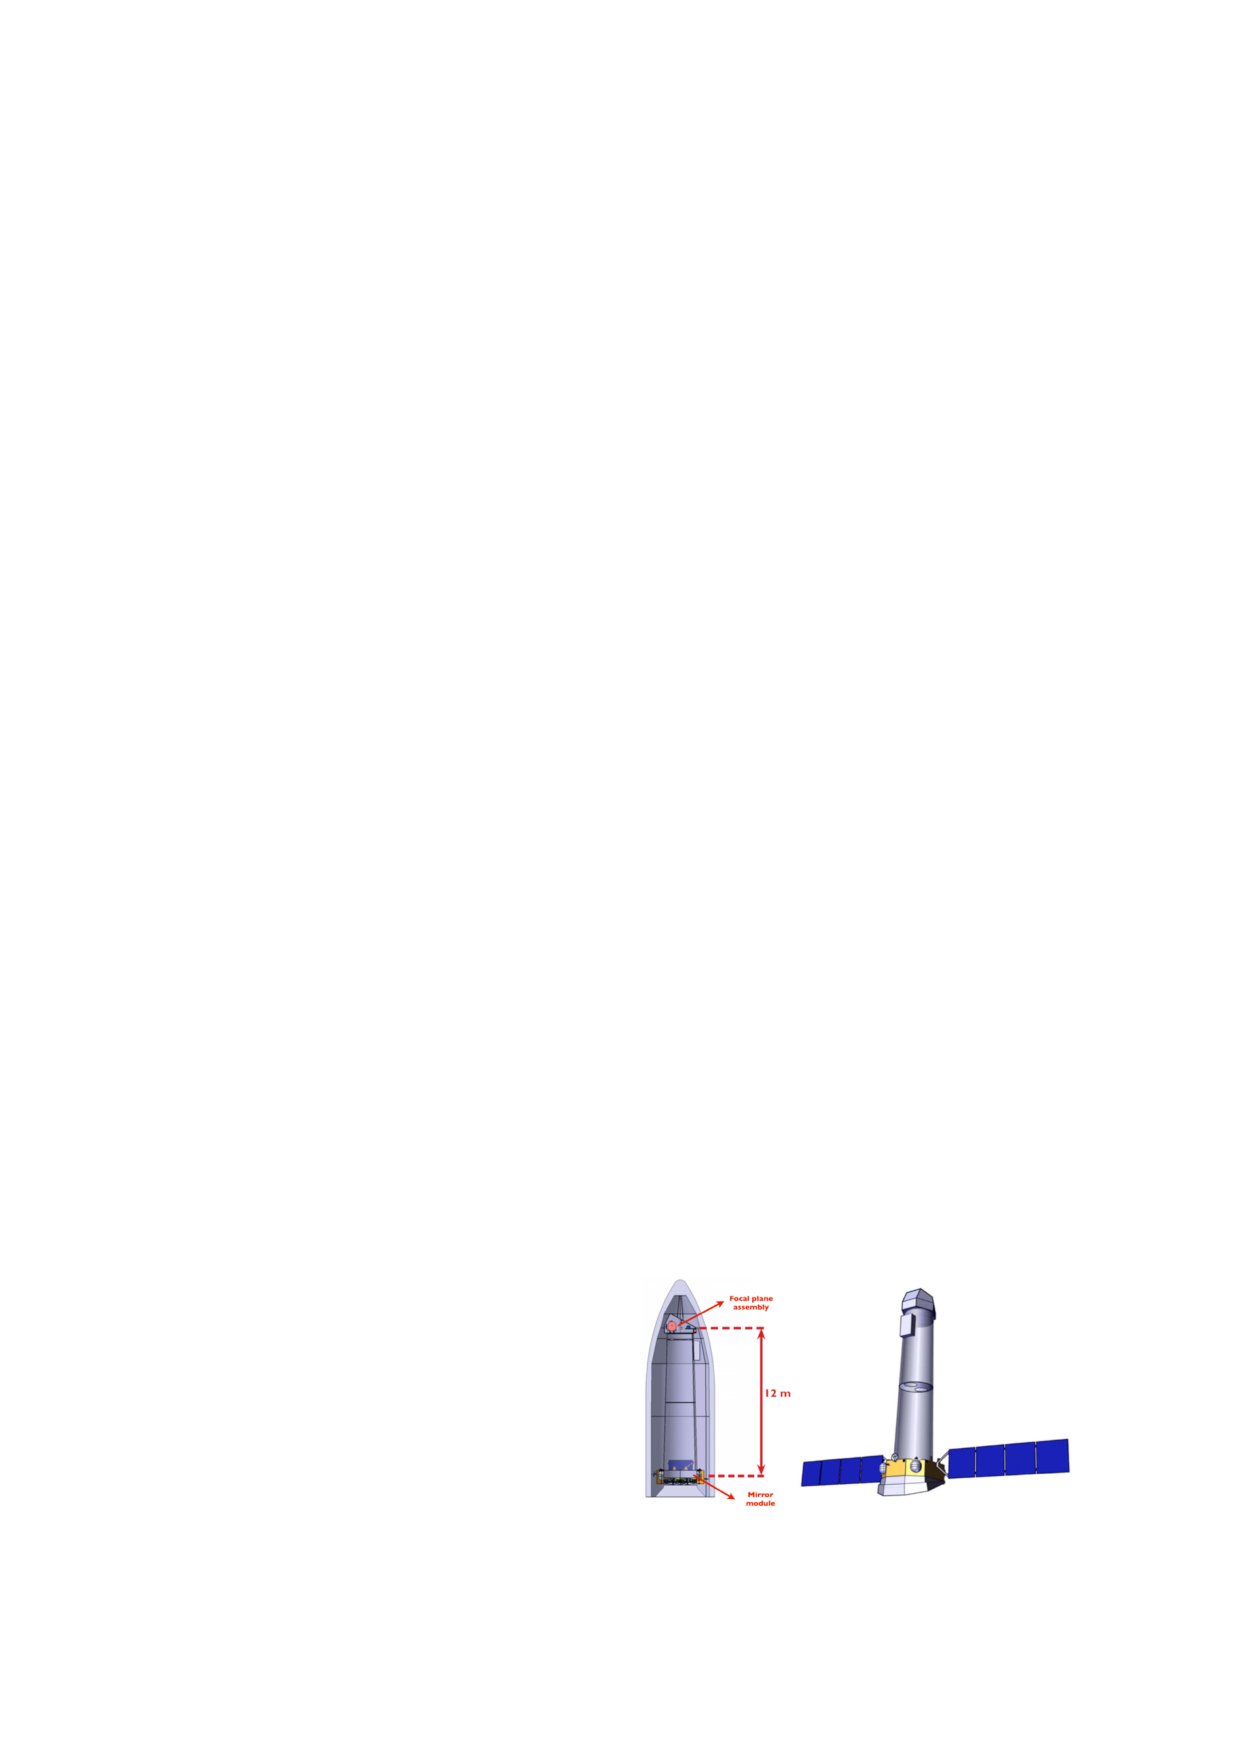
\includegraphics[height=5cm]{figures/athena/athena_telescope.pdf}
\caption{\footnotesize Illustrations of the ATHENA X-ray telescope. \textbf{Left:} Inside Ariane V fairing. \textbf{Right:} In space with extended solar panels. The optic is in the bottom end. (from \url{www.the-athena-x-ray-observatory.eu}).}\label{fig:athena_telescope}
\end{figure}

The theme of the 2028 L2 mission is \emph{The Hot and Energetic Universe}, which calls for spatially resolved X-ray spectroscopy and deep wide-field X-ray spectral imaging. The performance should greatly exceed instruments currently in use such as Chandra and XMM-Newton as well as future mission such as Astro-H and eRosita. The improvements are to be realised with an effective area of 2 m$^2$ at 1 keV, 5'' angular resolution and 40'x40' wide field-of-view\cite{Willingale:2013vo}.

\subsection{ATHENA optics technology}\label{sec:athena_opt_tech}
ESA has for the past decade been working on a radically new optics technology for future X-ray missions, the Silicon Pore Optics (SPO)\cite{Barcons:2012va}. By using silicon wafers, cut into rectangular shapes (diced) and with grooves cut into the underside, a high collecting area can be achieved with very low mass and at the same time achieve angular resolution better than glass.

\begin{figure}[!h]
  \center
  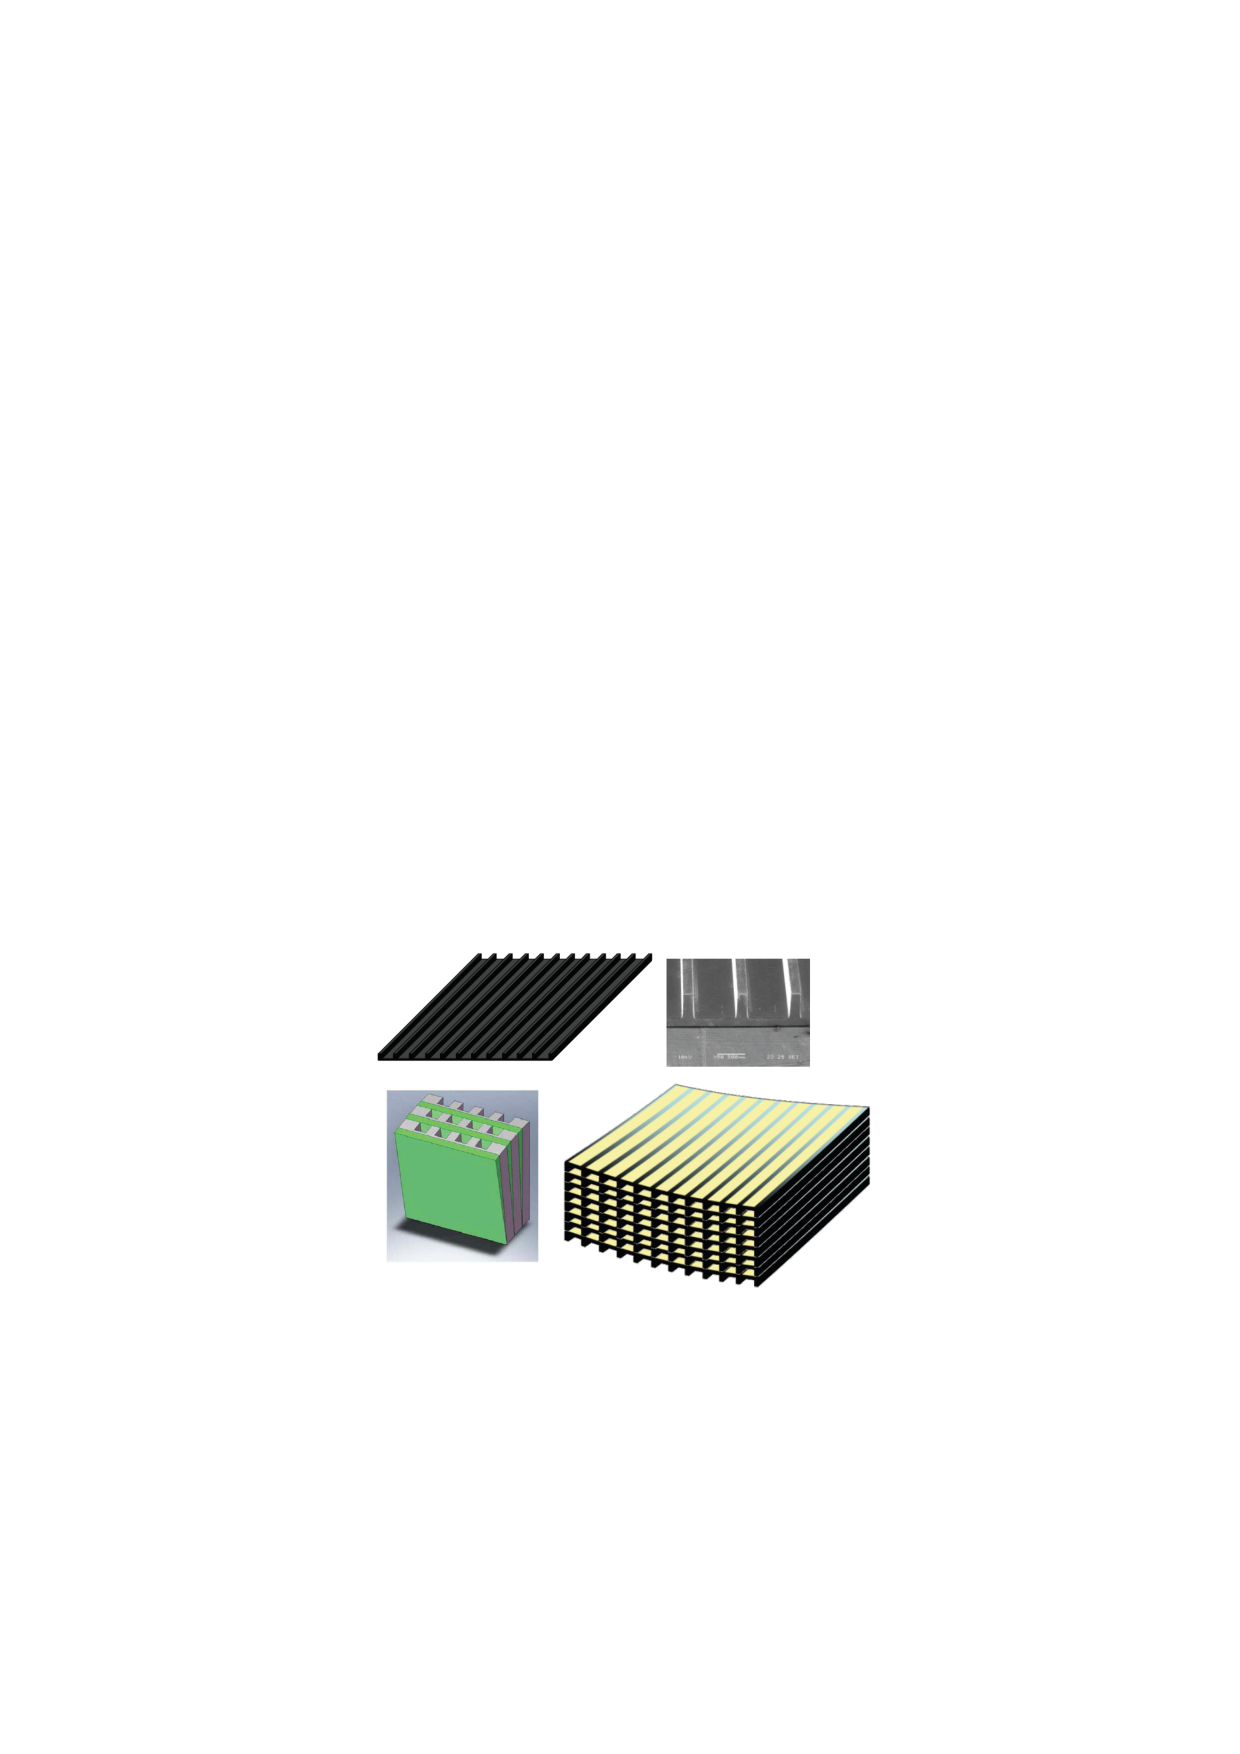
\includegraphics[height=6cm]{figures/athena/spo_principle1.pdf}
\caption{\footnotesize Principles of the Silicon Pore Optic (SPO) technology. \textbf{Top:} Silicon wafers are diced into rectangular pieces and grooves are cut in the underside. \textbf{Bottom left:} The wafers have a wedge applied with SiO$_x$ and are stacked so all SPO substrates reflect to the same point. \textbf{Bottom right:} SPO substrates are stacked at a curvature corresponding to the radius at which they are placed in the optic. A reflective coating is applied in stripes on each substrates. (from \cite{Willingale:2013vo}).}\label{fig:spo_principle1}
\end{figure}

% \begin{figure}[htbp]
% \centering
% \begin{minipage}{.47\textwidth}
%   \centering
%   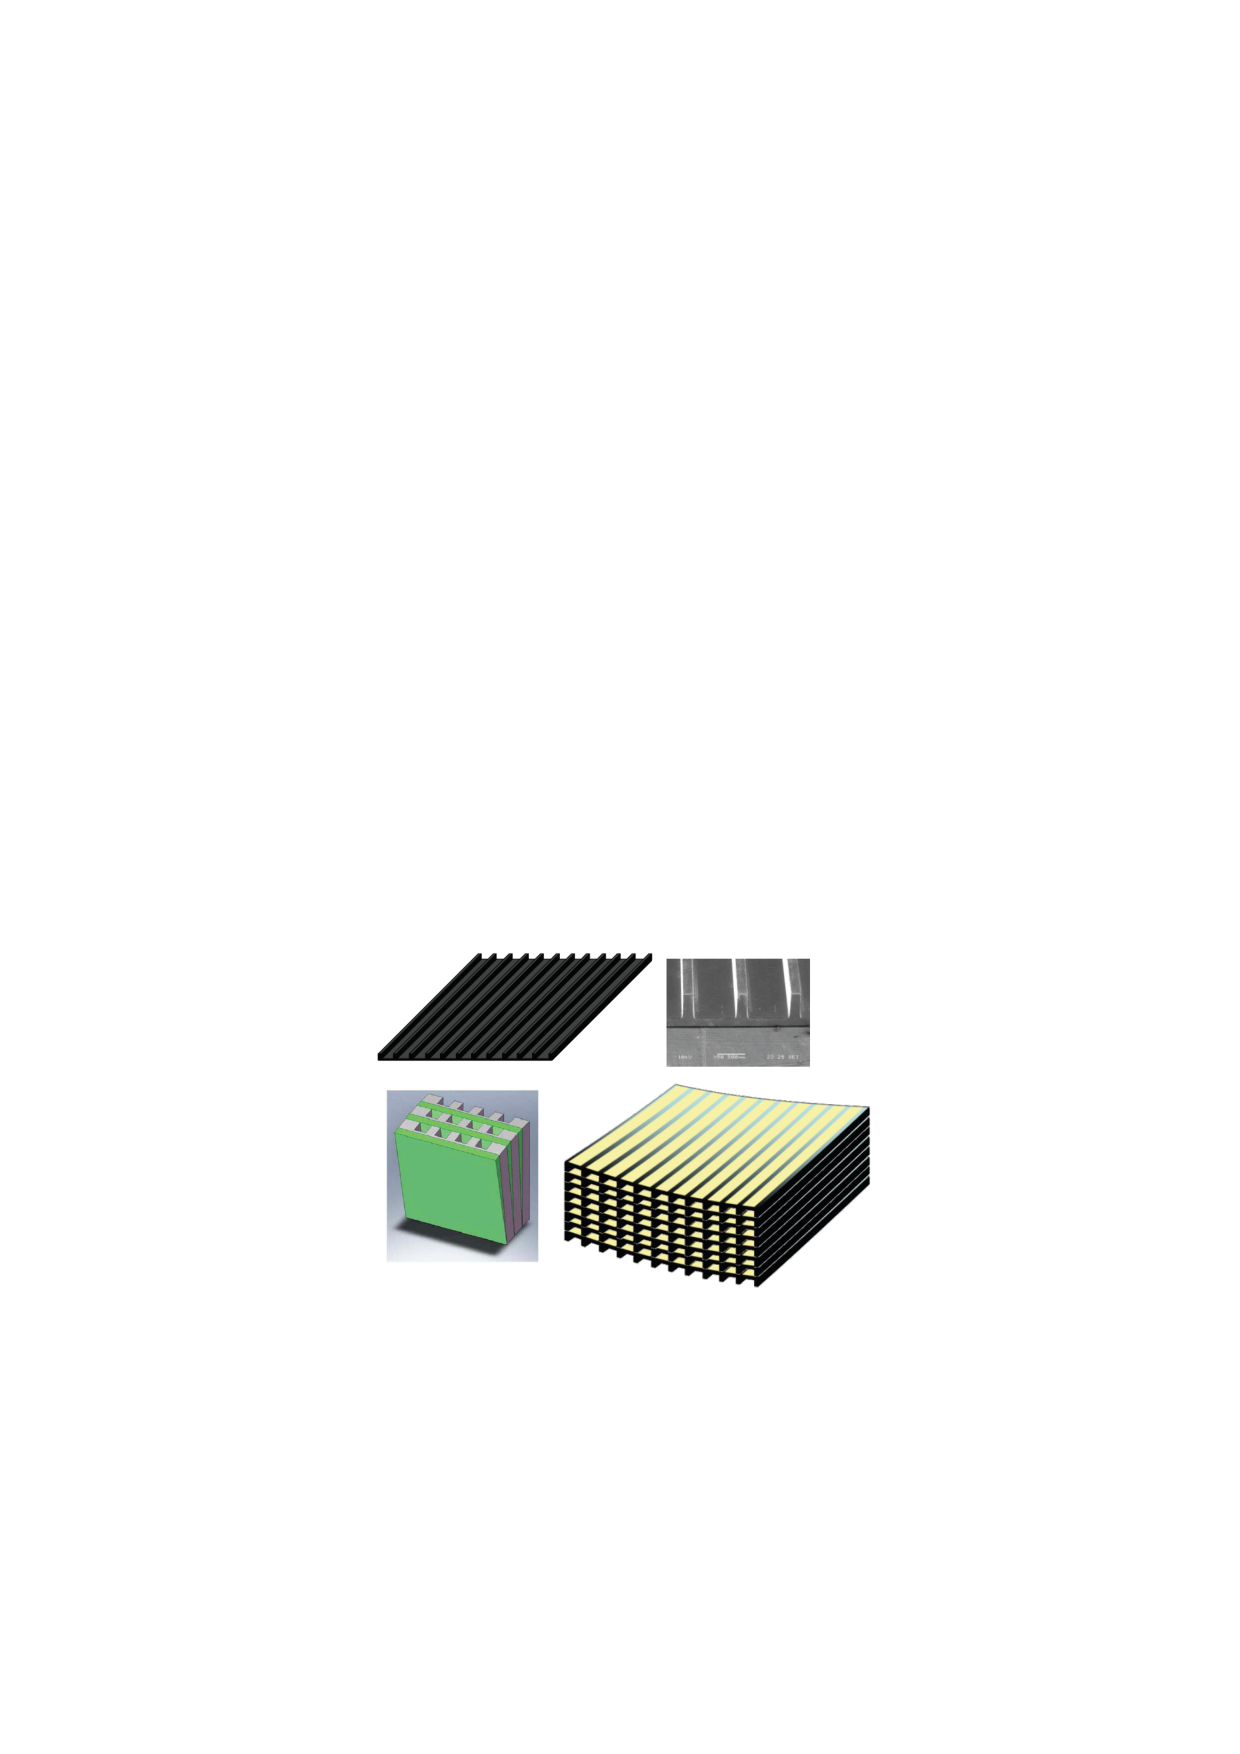
\includegraphics[width=\linewidth]{figures/athena/spo_principle1.pdf}
%   \captionof{figure}{\footnotesize  (from \cite{Willingale:2013vo}).}
%   \label{fig:spo_principle1}
% \end{minipage}%
% \hspace{20pt}
% \begin{minipage}{.47\textwidth}
%   \centering  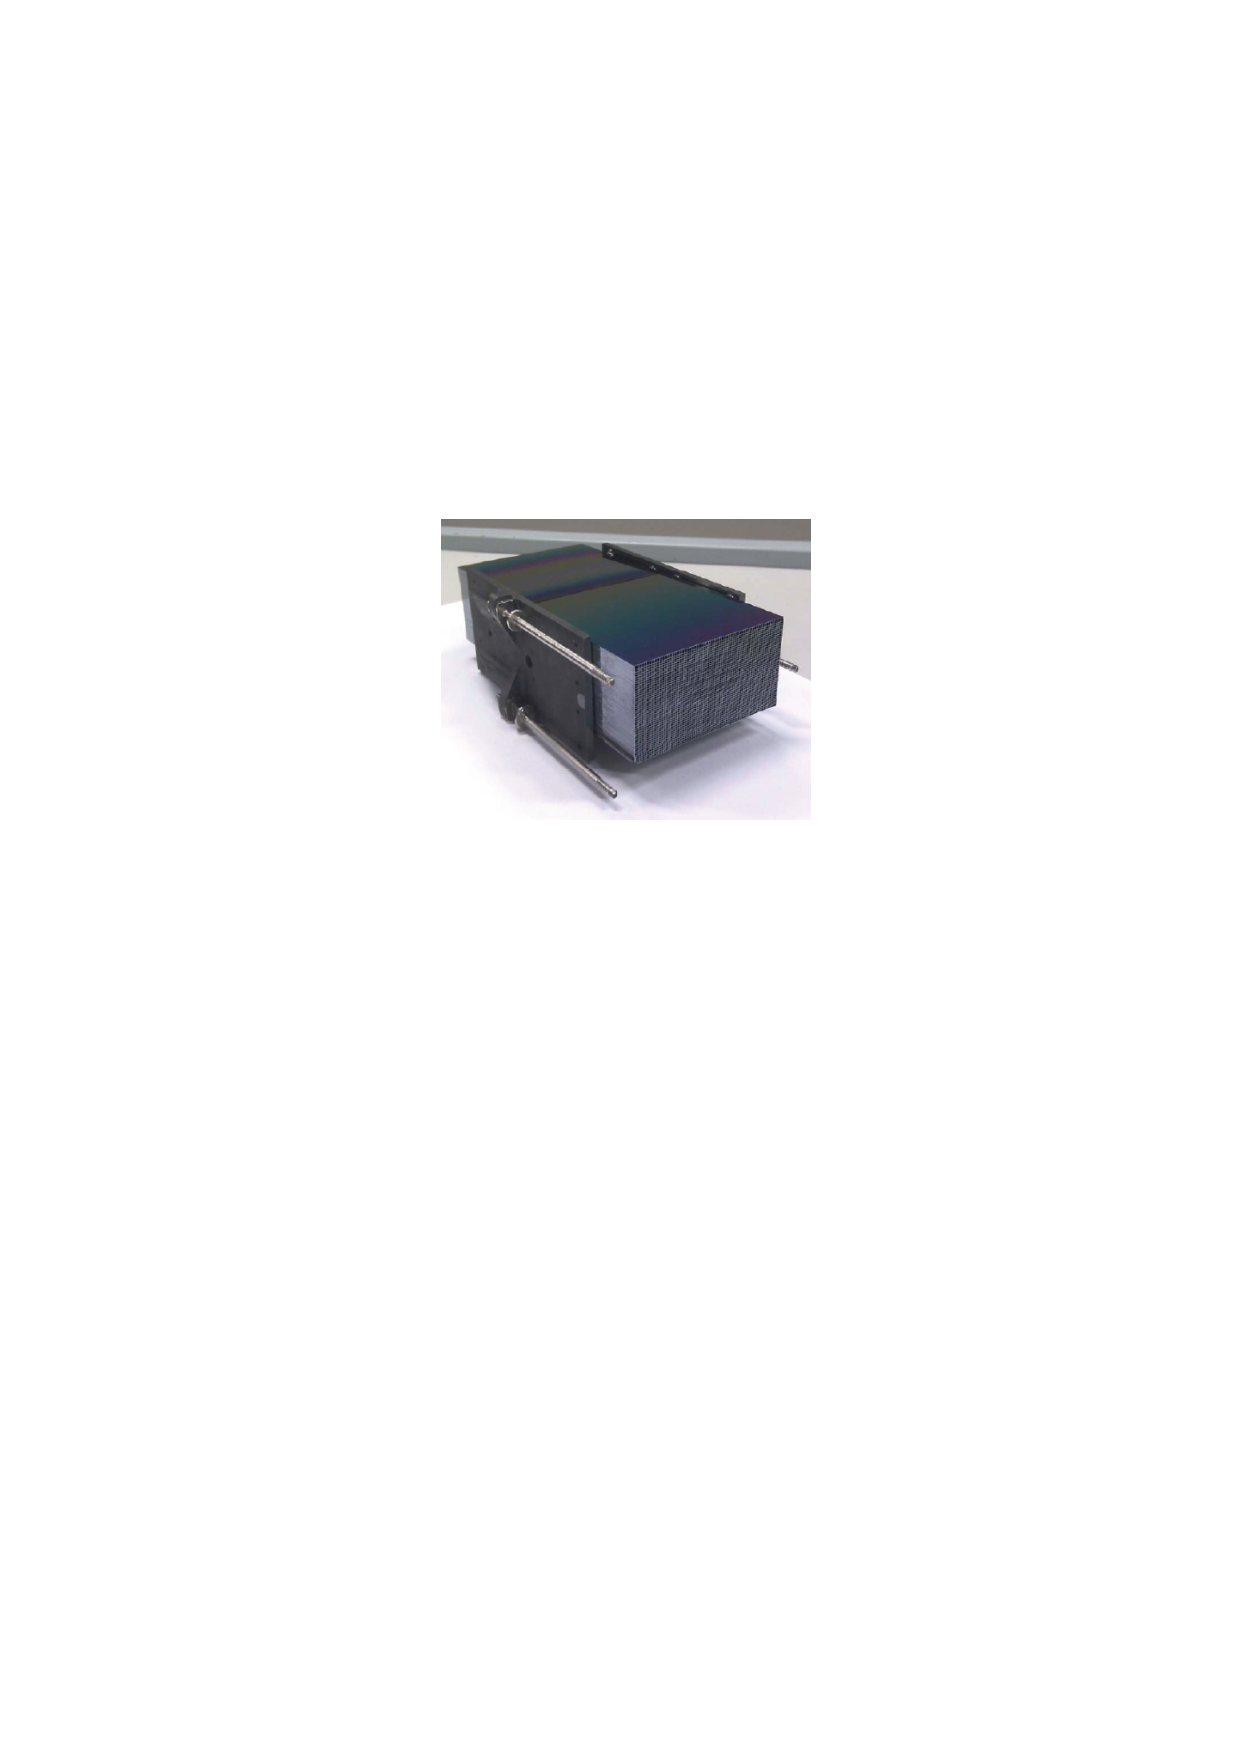
\includegraphics[width=\linewidth]{figures/athena/spo_stack.pdf}
%   \captionof{figure}{\footnotesize }
%   \label{fig:spo_stack}
% \end{minipage}
% \end{figure}

The silicon wafers are diced, wedged and grooves are cut into the underside, see figure \ref{fig:spo_principle1}. The grooves are 0.83 mm wide and spaced only 0.17 mm apart, resulting in narrow ribs in the underside. The grooving has two purposes: First, the wafer becomes so thin that it is bendable transversely to the ribs. Second, the SPO substrates can be stacked directly on top of one another with the ribs bonding to the surface of the substrate underneath. The X-rays will the be able to pass between the ribs and reflect on the surface of the bottom substrate. Stacking 68 of the SPO wafer substrates results in a very light, but very rigid block of silicon with micro-pores and a reflecting surface inside each pore. In order to have the SPOs reflect photons to the same spot, a wedge is applied to each reflecting surface corresponding to the angle required, see figure \ref{fig:spo_principle1} bottom left. The wedge is made from SiO$_x$ that is etched to the correct thickness and slope.

As the SPO substrates can be bend, they are stacked on a mandrel with the exact curvature needed. The high-precision stacking process is done by a dedicated robot in a controlled ultra-clean environment, as single dust specks can offset the stacking precision.

Two stacks of 68 SPO substrates constitutes an SPO module as can be seen in figure \ref{fig:spo_stack}. Each stack will reflect an incoming X-ray photon once, so two stacks acts like a conical approximation to the double-reflection Wolter I optic. However, in order to achieve sub-10'' angular resolution as specified by the science-criteria for ESA, the SPO technology will need to achieve a true Wolter I shape. Several initiatives by ESA are underway to achieve this as of 2014.

\begin{figure}[!h]
  \center
  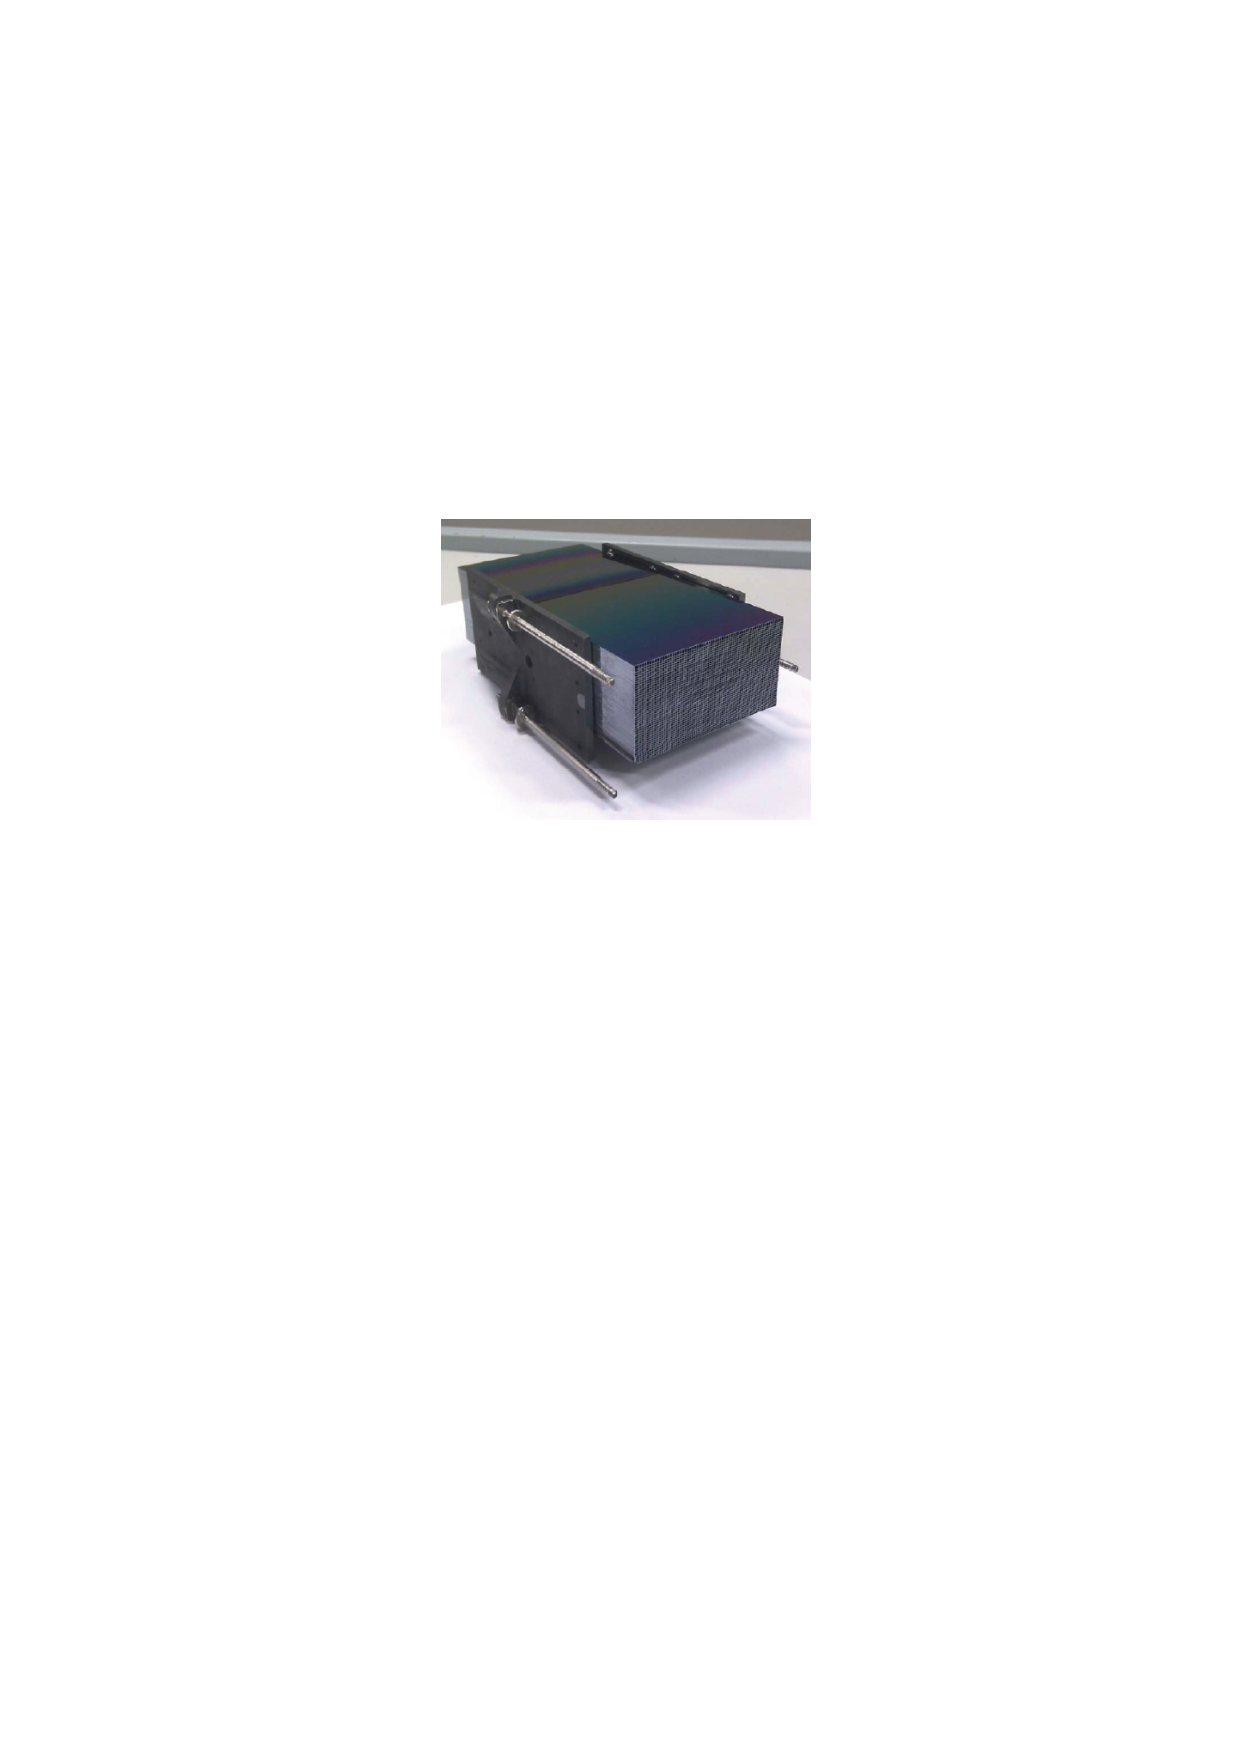
\includegraphics[height=6cm]{figures/athena/spo_stack.pdf}
\caption{\footnotesize A complete SPO mirror module. Two stacks of 68 SPO substrates are glued together with a pair of Cesis plates, making them co-aligned with 1'' precision. The complete module reflects an incoming X-ray photon twice and thus acts as both paraboloid and hyperboloid of the Wolter I optic. (from \cite{Willingale:2013vo}).}\label{fig:spo_stack}
\end{figure}

Each SPO module is self-consistent, making the entire optic technology modular. When a module is ready, it can be slided into a light-weight construction. This is in contrast to the NuSTAR technology where each layer had to be mounted sequentially. The modularity is also a necessity when it becomes apparent that an effective area of 2 m$^2$ at 1 keV requires 1.5 mil. pores. As ATHENA is a large ESA mission, the Ariane V rocket will be used and the telescope is designed with the size limitations of the Ariane V fairing in mind, resulting in a telescope with $\sim$3 m diameter and $\sim$13 m length. To populate an optic with a diameter of $\sim$3 m, the number of SPO modules needed are $\sim$900 as can be seen in figure \ref{fig:athena_full_optic}.

\begin{figure}[!h]
  \center
  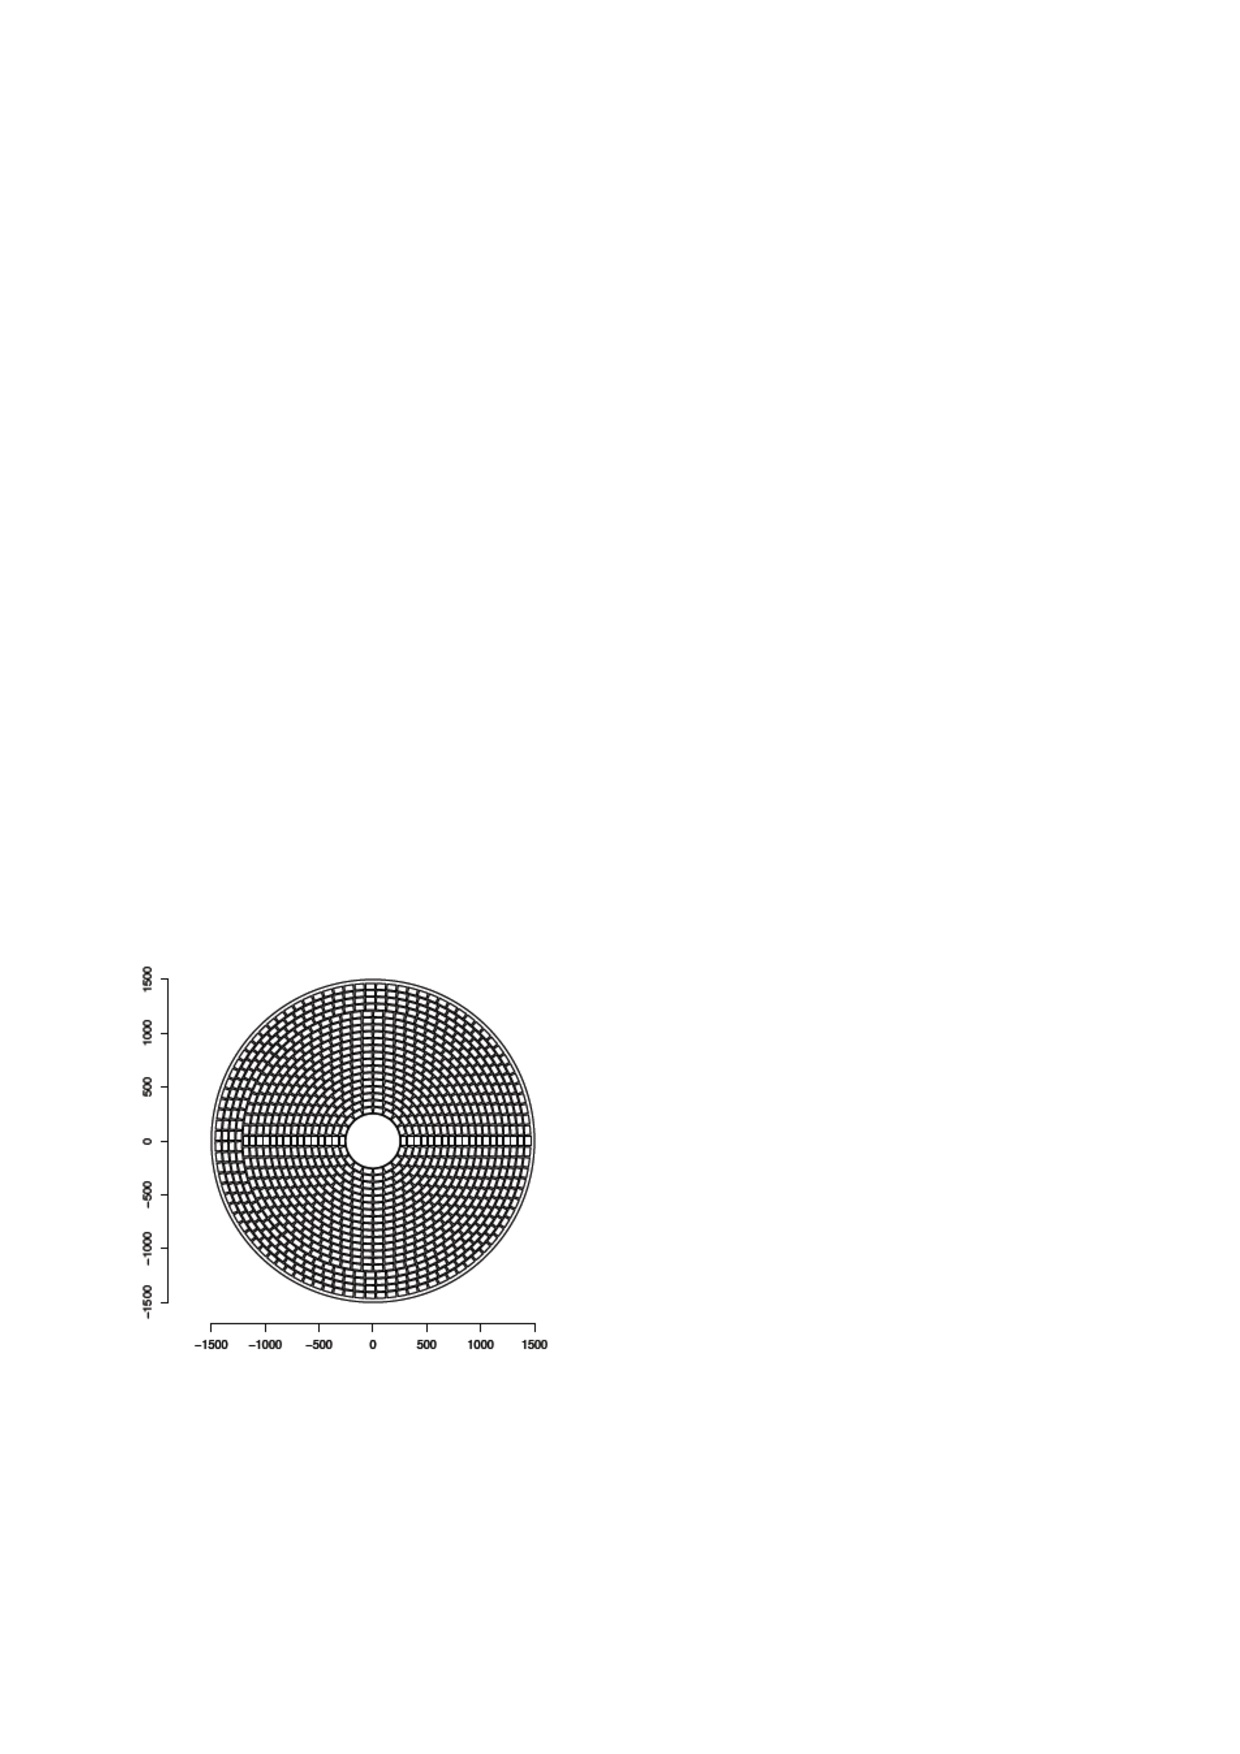
\includegraphics[height=6cm]{figures/athena/athena_full_optic.pdf}
\caption{\footnotesize The complete ATHENA optic. SPO mirror modules are arranged in rings to populate the aperture. (from \cite{Willingale:2013vo}).}\label{fig:athena_full_optic}
\end{figure}

As each optic module consist of $2 \cdot 68 = 136$ SPO substrates, a total of $900 \cdot 136 \approx 123,000$ SPO substrates are needed, not accounting for spares or broken substrates. Considering that the NuSTAR telescope consisted of $2\cdot2376$ glass substrates and took two years to produce, it becomes apparent that the ATHENA mission will require a large-scale production facility. In section \ref{sec:athena_upscaled} can be found an investigation in the coating side of the production facility requirements for the original ATHENA mission proposed for the ESA L1 mission. It consisted of two optics with a total of 64,640 SPO substrates.

\subsection{Reflective coatings on SPO substrates}
One of the most important principles of the SPO technology is the ability for the SPO substrates to bond when stacked. It is achieved by pressing the surface of one SPO substrate against the ribs of another SPO substrate. Since the SPO substrates are wedged with a SiO$_x$ material, both ribs and surface consist of SiO$_x$ and pressing the two substrates together forms a strong covalent bond, thereby fusing the two.

In order to apply a reflective coating to each of the SPO substrates, the bonding process has to be taken into account. Applying a coating with a physical vapor deposition process such as DC magnetron sputtering will coat the whole surface, but by using a lithographic process from the semiconductor industry it is possible to apply coatings in patterns on a surface. The pattern being the exact position where the ribs will touch the surface when stacking, so these areas are $\sim$0.17 mm wide, covers the entire length of the substrate surface and are spaced $\sim$0.83 mm apart. The lithographic process involves the following (also seen in figure \ref{fig:litho_process}):

\begin{itemize}
  \item Applying a resist film on the substrate surface.
  \item Curing the resist with e.g. a UV light in a striped pattern corresponding to the ribs of the SPO substrate.
  \item Removing the un-cured resist with a chemical solution (the developer).
  \item Coating the substrate with a reflective coating.
  \item Removing the cured resist including the coating applied on top of the resist using acetone or DMSO\footnote{Dimethyl sulfoxide}.
\end{itemize}

\begin{figure}[!h]
  \center
  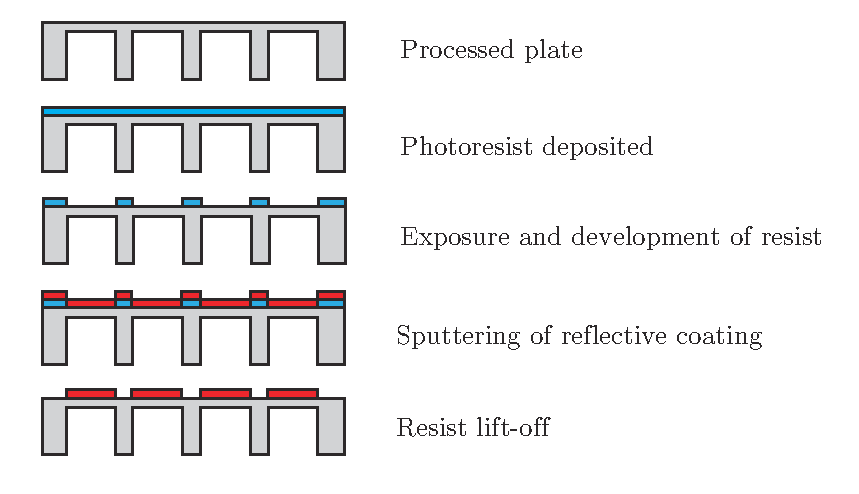
\includegraphics[height=6cm]{figures/athena/litho_process.pdf}
\caption{\footnotesize. The lithographic process applied to SPO substrates to achieve a striped pattern of reflective coating.}\label{fig:litho_process}
\end{figure}

The lithographic process puts requirements on the reflective coatings applied to the SPO substrates since chemical solutions used in the last step are designed to break carbon-carbon bonds. All multilayer coatings with pure C as the low-Z material are excluded as the last step described above will simply break apart the coating.

\subsection{The ATHENA reflective coating baseline}
The baseline coating for ATHENA is a Ir/B$_4$C single bilayer. The Ir will reflect higher energy X-rays in the 0.1--10 keV energy range, and the B$_4$C top layer will reflect lower energies. The B$_4$C material is able to withstand the C-C bond-breaking chemical solutions applied in the last step of the lithographic process, while at the same time being a very light material. The low electron density gives B$_4$C a very good reflectivity at energies 0.1--$\sim$3 keV.

The Ir/B$_4$C combination does however have some drawbacks, especially high compressive film stress. Additionally, the thin film material combination is not described in the litterature, so the interplay between the two materials in both the short and long term is relatively unknown. In appendix \ref{pap:PREL_ATHENA} can be found a paper from 2011 that investigates the baseline ATHENA coating along with solutions to handle the film stress. In section \ref{sec:athena_cr_impro} is a continuation of the investigation into stress improvements.

\subsection{Coating optimisations for ATHENA}
To improve on the ATHENA baseline coating, a range of alternative material combinations were investigated using computer optimisation with Markov-Chain Monte-Carlo methods by Desiree D. M. Ferreira at DTU Space. A number of optimised coating recipes were produced for each material combination and the actual coatings were subsequently produced on SPO substrates in the coating lab at DTU Space. In appendix \ref{pap:athena_2012} can be found a paper from 2012 on some of the optimizations and investigations done on coatings applied to SPO substrates.

\section{Investigation of Cr roughness improvement}\label{sec:athena_cr_impro}
The baseline coating for ATHENA consists of a bilayer of Ir and B$_4$C, the former of which shows considerably film stress of up to -4 GPa (compressive). To alleviate the stress in the film, earlier investigations has shown significant improvements in stress by using a Cr underlayer, which almost eliminates the total film stress[\ref{pap:PREL_ATHENA}].

The drawback is however the high surface roughness in Cr films. We present here the results of two experiments with the purpose of reducing the Cr surface roughness. The first experiment is an attempt to decrease the rate of sputtered Cr atoms reaching the substrate. A lower rate will give an adsorbed Cr atom a chance to move to a lower position\cite{Venables:1984wu}. By decreasing the output power to the Cr cathode, while maintaining the same voltage of -400 V, the rate of sputtered atoms can be decreased. In figure \ref{fig:cr-power-change} XRR measurements of Cr films coated at varying power output can be seen.

\begin{figure}[!h]
	\center
	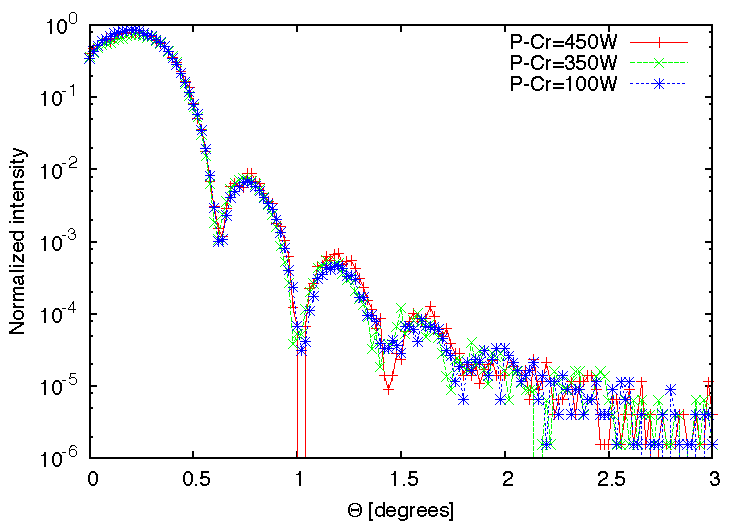
\includegraphics[height=6cm]{figures/athena/coatings/cr-power-change.pdf}
\caption{\footnotesize XRR measurements of four Cr single layer coatings made with varying power settings.}\label{fig:cr-power-change}
\end{figure}

It is seen that at lower power settings, the hills and fringes become less pronounced, indicating a higher roughness. This would indicate that the flux of sputtered atoms adhering to the substrate have time to coalesce into islands, thereby giving rise to island-growth also known as \emph{Volmer-Weber} growth\cite{Thompson:2000ge}. In that case, it would seem that lowering the power on Cr yields a higher surface roughness because given enough time, the Cr adatoms will form into their preferred configuration.

A second experiment involves changing the Ar gas pressure during coating. A minimum pressure is required in order to sustain the cathode plasma, but it is beneficial to coat at the lowest possible pressure. At a given pressure, the sputtered atoms going from target to substrate will have a chance of hitting an Ar atom given by the mean free path. A sputtered atom that would otherwise hit the substrate at a very low normal angle, will after having hit an Ar atom reach the substrate at a much higher angle, thereby giving rise to shadow-effects\cite{Barabasi:XbjHWFWZ} as seen in figure \ref{fig:self-shadow}.

\begin{figure}[!h]
	\center
	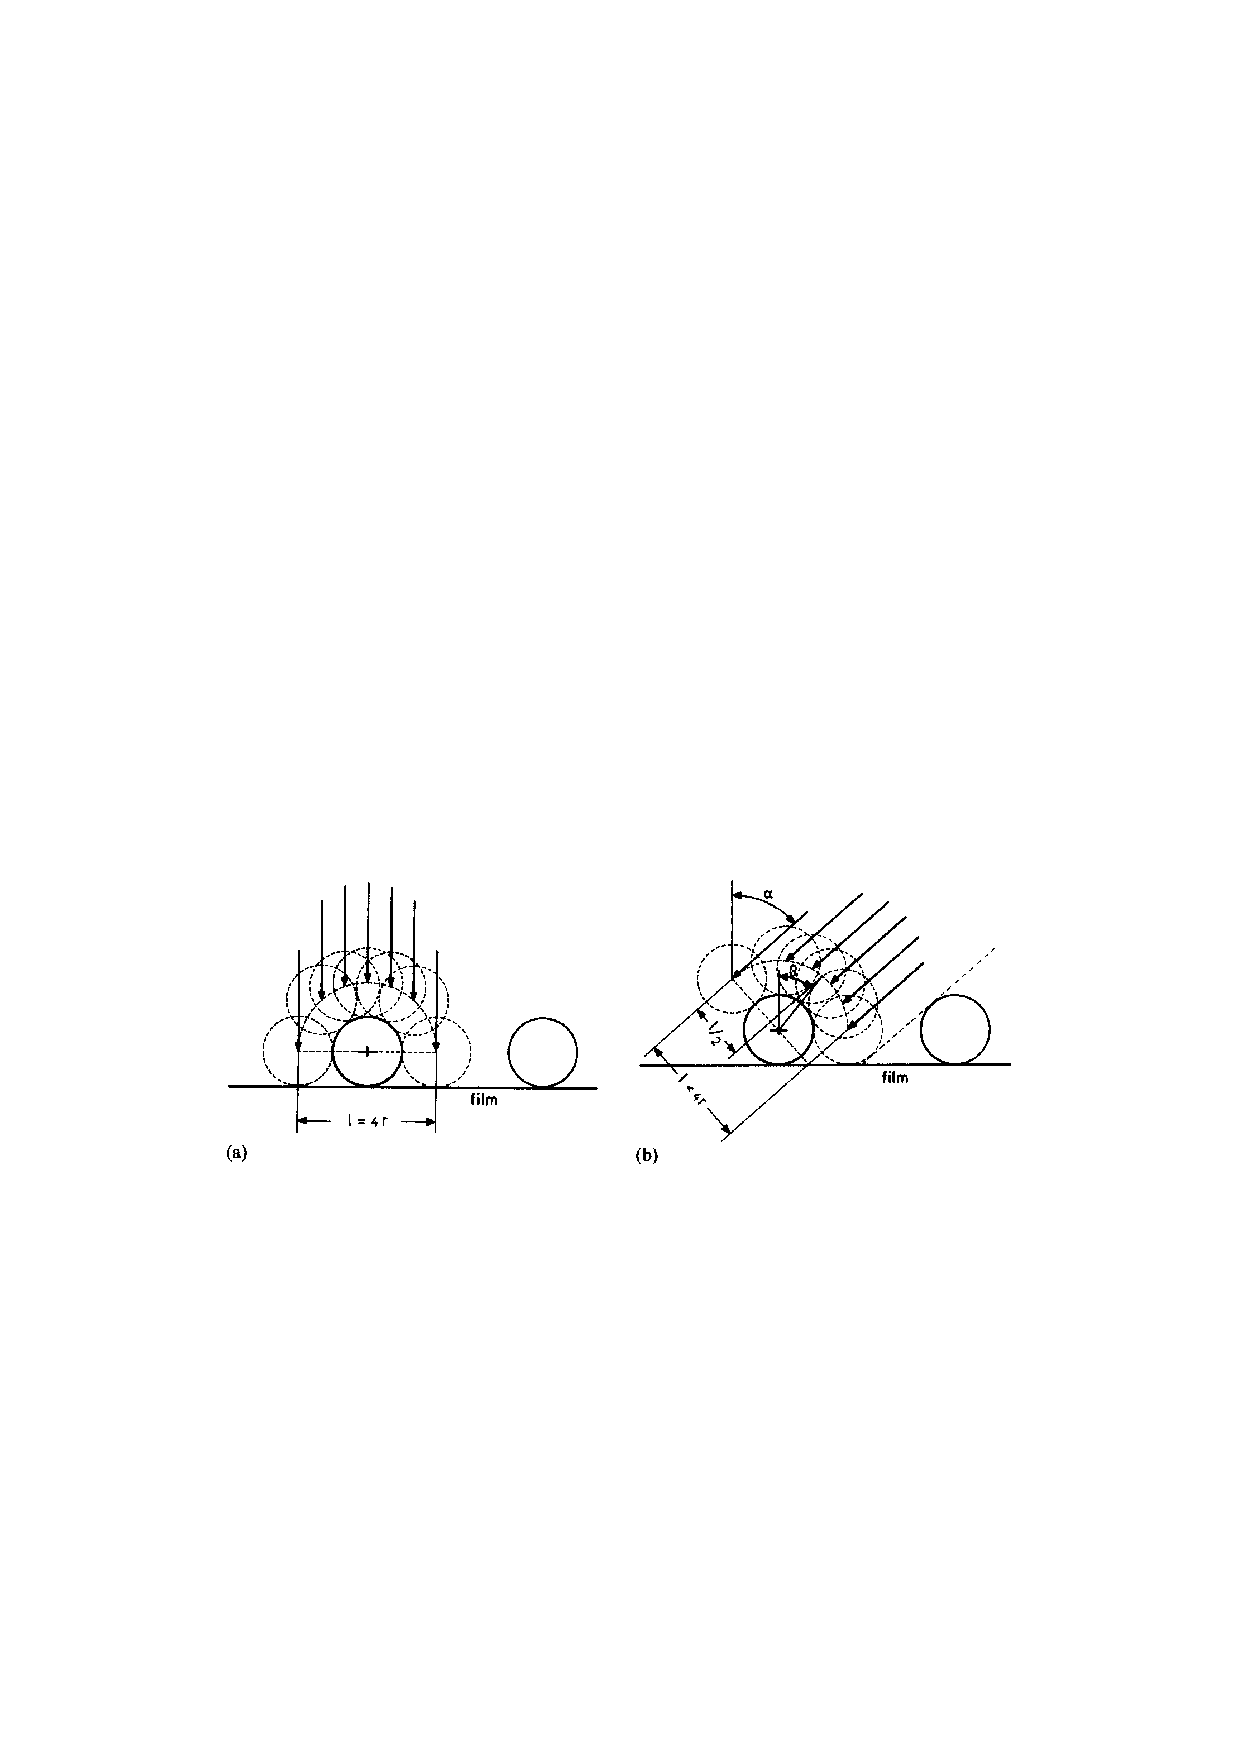
\includegraphics[height=3.5cm]{figures/athena/coatings/self-shadow.pdf}
\caption{\footnotesize Principle of self-shadowing during angled deposition on a surface. At higher angles, incoming particles will have a tendency to adsorb on top of single particles already on the surface instead of filling gaps in the film. From \cite{Dirks:1977uk}.}\label{fig:self-shadow}
\end{figure}

By producing Cr coatings at varying Ar pressures and measuring using XRR, a correlation was found between Ar pressure and Cr surface roughness. The XRR measurements along with IMD fits can be seen in figure \ref{fig:cr-pressure-fit}. A decrease in Cr surface roughness from 1.0 nm to 0.7 nm is seen when going from 2.4 mTorr to 1.5 mTorr Ar pressure.

\begin{figure}[!h]
	\center
	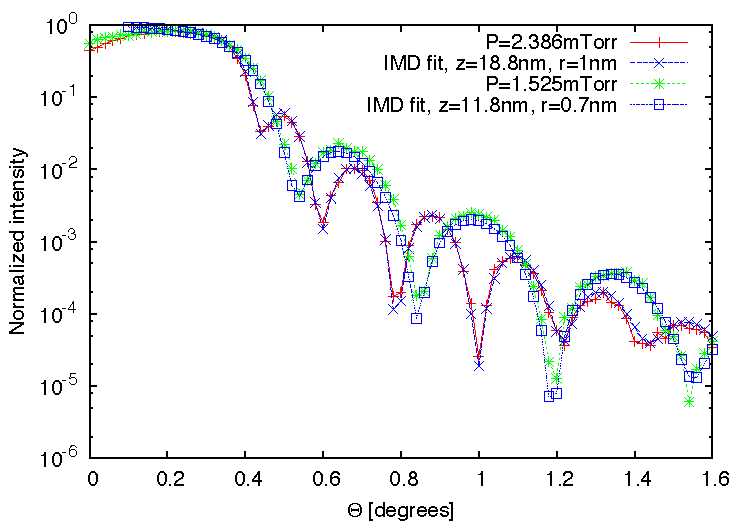
\includegraphics[height=6cm]{figures/athena/coatings/cr-pressure-fit.pdf}
\caption{\footnotesize XRR measurements of two Cr single layer coatings made with varying Ar pressure. Blue points are IMD models fitted to the data.}\label{fig:cr-pressure-fit}
\end{figure}

Earlier investigations of the baseline Ir/B$_4$C coating with Cr sublayer\cite{Jakobsen:2011vd} have hinted that the interface roughness of Ir/B$_4$C becomes lower than the interface roughness of Cr/Ir. A simple bilayer coating of Cr/Ir have now been made, where B$_4$C can be factored out of the fitting procedure. The B$_4$C has been left out, so to easier constrain the surface roughness of Ir and Cr in the fitting process as the model only has 4 variables compared to 6 variables for a Cr/Ir/B$_4$C coating. The coating was made using the standard Ar pressure of 2.9 mTorr. XRR measurement of the sample can be seen in figure \ref{fig:cr-ir-fit} along with a an IMD fit. The fitted curve shows a Cr/Ir interface roughness of 0.62 nm and an Ir surface roughness of 0.3 nm.
This is an extremely promising result, since the baseline ATHENA coating depends on the Ir surface for most of the energy response above $\sim$3 keV. So to have this surface smooth while at the same time keeping a low amount of film stress is reassuring.

\begin{figure}[!h]
	\center
	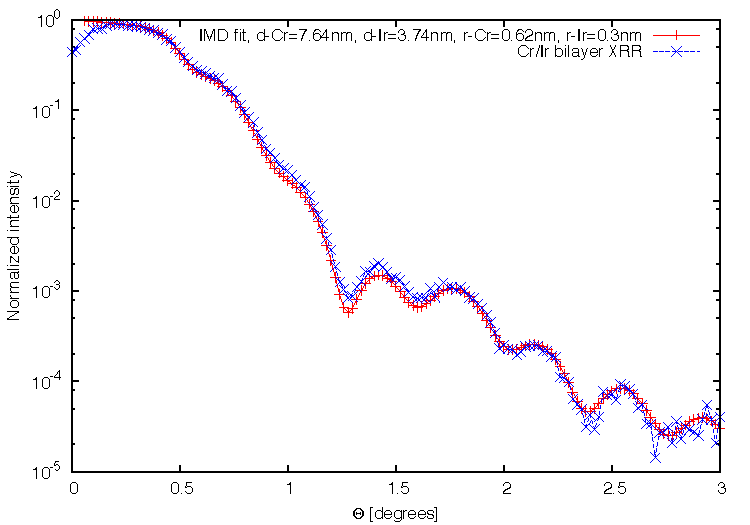
\includegraphics[height=6cm]{figures/athena/coatings/cr-ir-fit.pdf}
\caption{\footnotesize XRR measurement of a bilayer of Cr/Ir (red) along with an IMD model fitted to the data (blue).}\label{fig:cr-ir-fit}
\end{figure}

\section{Investigation of pulsed-DC sputtering}
We investigate the use of pulsed sputtering to decrease roughness as thickness increase as described in the litterature\cite{Pei:2009gn,Shaha:2011gy,Turkin:2010ur}. In the paper by Pei et al, a sputtering cathode with a C target was supplied with -400 V and 1.5 A at 350 kHz and 50\% duty cycle. The substrate was place 10 cm away from the target and supplied with -40 V at 250 kHz at 50 \% duty cycle. The high frequency at the target allows for a much higher percentage of the sputtered atoms to become ionized, giving them a positive charge. At regular non-pulsed DC sputtering, only 10 \% are ionized atoms, but for pulsed that increases to 60-70 \%\cite{Bradley:2002ge,Pei:2008jl}. The negative pulsed bias on the substrate will pull in the ionized sputtered atoms at much higher velocity than possible for DC sputtering. The higher velocity sputtered atoms gives rise to denser and more smooth films, as the momentum of the impact causes a temporary 'liquidification' of the immediate surrounding thin film on the nano-scale.

Attempts by Pei et al show promising results for decreasing interlayer roughness in multilayers using a high frequency pulse modulation on the power delivered to the cathode with lighter material, in their case carbon was used. For coatings for the ATHENA mission, it is critical to use B$_4$C as the light material, as a regular C layer will be dissolved in the lift-off process that removes the lithographic resist.

We acquired the same power supply, an Advanced Energy Pinnacle Plus+ 5+5 capable of delivering two channels of 5 kW at 350 kHz. Using W and B$_4$C, 10 bilayer coatings were produced with the same power supply setup as mentioned in \cite{Pei:2009gn}. The entire rotating ring in the multilayer coating chamber at DTU Space is designed to hold a separate bias or be grounded depending on configuration. Initial results can be seen in fig. \ref{fig:wb4c-pulsed}.

\begin{figure}[!h]
	\center
	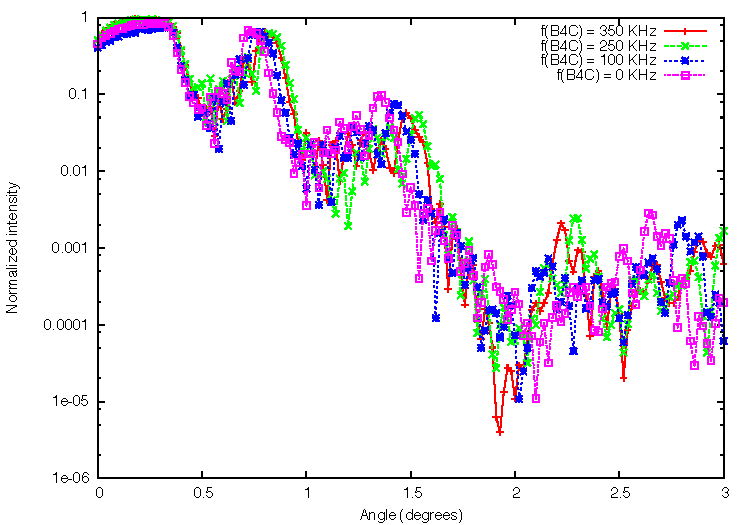
\includegraphics[height=6cm]{figures/athena/coatings/w-b4c_pulsed.pdf}
\caption{\footnotesize XRR measurements of four W/B$_4$C 10 bilayer films made with varying pulsed-DC frequency on the B$_4$C cathode.}\label{fig:wb4c-pulsed}
\end{figure}

The figure show XRR measurements of 4 samples coated with 10 bilayer W/B$_4$C with different frequencies supplied to the B$_4$C target. For a 10 bilayer coating, we expect to see clear Bragg peaks with 8 Kiessig fringes between, but all samples show washed out 1st and 2nd order Bragg peaks and an indeterminate number of Kiessig fringes. Even the sample coated without a pulsed B$_4$C cathode show the same behavior. In figure \ref{fig:wb4c-nopulsed}, the two samples coated with 350 kHz and 0 kHz in the same coating run is compared to a sample from a different run coated with regular DC sputtering showing well-defined Bragg peaks as would be expected.

\begin{figure}[!h]
	\center
	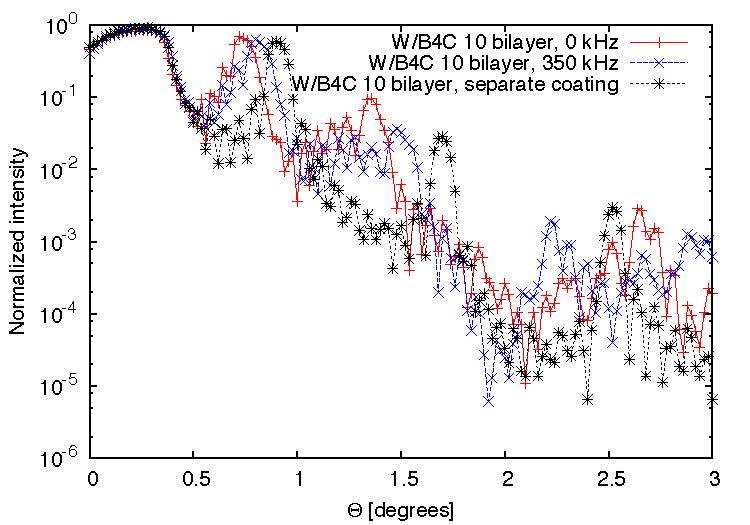
\includegraphics[height=6cm]{figures/athena/coatings/w-b4c-nopulsed.pdf}
\caption{\footnotesize XRR measurements of three W/B$_4$C 10 bilayer films. Two (red and blue) made using pulsed-DC sputtering and also shown in figure \ref{fig:wb4c-pulsed}. The last one (black) is made in a separate coating run without pulsed-DC sputtering, but otherwise with the same coating parameters.}\label{fig:wb4c-nopulsed}
\end{figure}

Something has clearly gone wrong in the pulsed-DC coating. The new software recently installed to control the multilayer coating chamber logs the cathode output every 5 seconds and a plot of that can be seen in figure \ref{fig:power-output}(left) compared to a log from a regular DC coating, figure \ref{fig:power-output}(right). The figure shows clearly that the power output to the B$_4$C cathode drops to zero in the middle of a rotation. The B$_4$C cathode should be at 900 W output for the entire time the W cathode is off.

\begin{figure}[!h]
	\center
	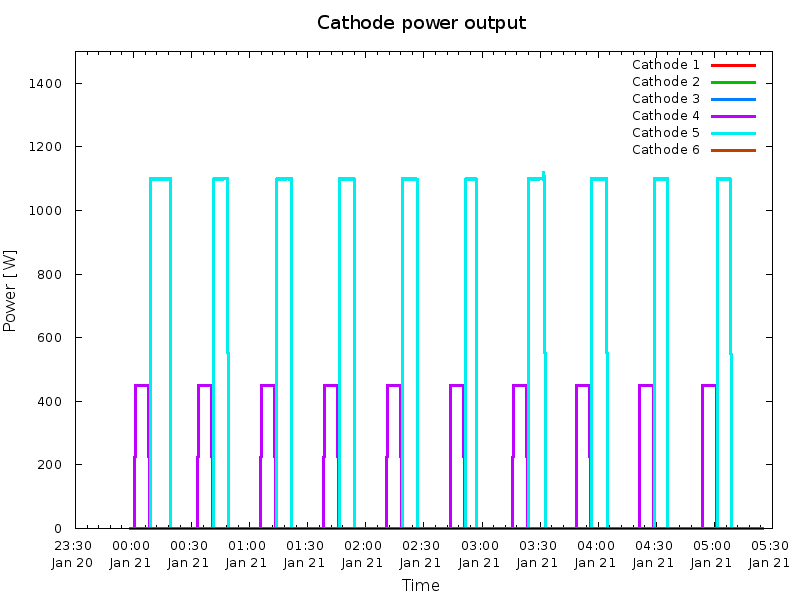
\includegraphics[width=0.47\linewidth]{figures/athena/coatings/power_output_rf_coating.png}
	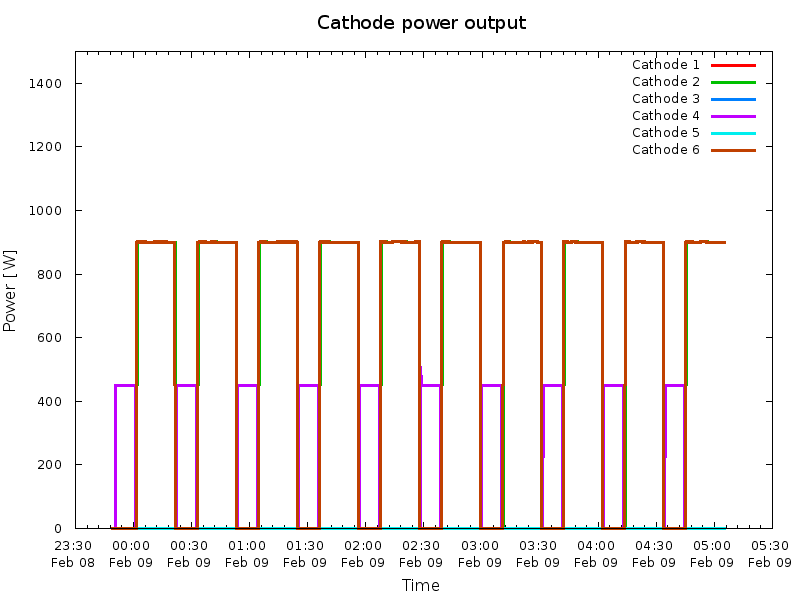
\includegraphics[width=0.47\linewidth]{figures/athena/coatings/power_output_dc_coating.png}
\caption{\footnotesize Graphs of cathode power output over time during a coating run. Left is from a W/B$_4$C 10 bilayer coated using pulsed-DC sputtering on the B$_4$C material. Right is from a W/B$_4$C 10 bilayer coating made without pulsed-DC sputtering.}\label{fig:power-output}
\end{figure}

It is not uncommon to see a cathode 'drop out' during a coating run, where the power supply is unable to sustain the plasma. In that case the power supply will increase the voltage to get the plasma to ignite again and the power output will in that period be 30-40 W. In this case the power output drops to zero, which is inconsistent with a conventional drop-out. Investigating the matter further shows that the 'arc'-protection system on the power supply goes off rapidly during a coating. Arcs are a sudden discharge from cathode to the grounded anode shield and can have a wide variety of causes. The arc-protection will protect the power supply from the power surge and will tell the user when it happens. The inner anode shield in the B$_4$C cathode clearly shows damage from arcing in the steel and the shielding teflon strips, which looks like welding marks. We assume that at some point during the coating, the damage creates enough debris to make a short between cathode and anode shield.

It is at this moment still unclear what causes the arcing. The pulsed-DC system brings many more variables into an already complicated sputtering process. The best assumption at the moment is either that the cables from power supply to cathode are too long or that a wire assembly box has insufficient electrical shielding.

\begin{figure}[!h]
	\center
	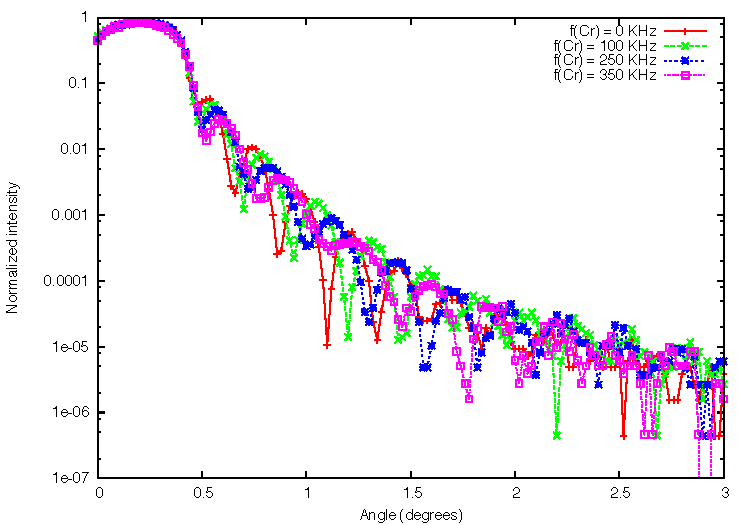
\includegraphics[height=6cm]{figures/athena/coatings/cr_pulsed.pdf}
\caption{\footnotesize XRR measurements of four samples coated with single layers of Cr using pulsed-DC sputtering at varying frequency. Sample coated with $f=0$ kHz (red) has a thickness of $\sim$17 nm. Sample coated with $f=350$ kHz (purple) has a thickness of $\sim$12 nm.}\label{fig:cr-pulsed}
\end{figure}

The second attempt at using the pulsed-DC method was with Cr single layer coatings. XRR measurements of the coated samples can be seen in figure \ref{fig:cr-pulsed}. Four samples were coated with varying frequencies applied to the Cr cathode. The measurements show clear differences in coated thickness between the frequencies used (position of Kiessig fringes does not overlap) and higher frequencies show a lower surface roughness (Kiessig fringes are less pronounced and shows a wavy pattern at the highest frequency). The XRR measurements were difficult to fit using IMD, indicating that the films are of non-uniform density. The coating done without pulsed-DC fitted to a $\sim$17 nm Cr thickness and the coating done with the highest frequency pulsed-DC sputtering fitted to a $\sim$13 nm Cr thickness. No arcing was seen when coating Cr using pulsed-DC sputtering.

We believe that the investigation of pulsed-DC sputtering have concluded with no improvements in the coatings. The arcing that was seen during pulsed-DC sputtering of B$_4$C, but did not show up for Cr, can have a variety of causes. First, the output power when coating B$_4$C is significantly higher than for Cr (1100 W compared to 450 W). The higher power puts higher demand on electrical shielding as well as the cable length between power supply and cathode. Second, there are fundamental differences in the two materials. The Cr is a well conducting and hard metal, whereas B$_4$C is not very well conducting and brittle. A very good contact is required between cathode and sputter material, but since the B$_4$C is very stiff and not as malleable as metal, the target can easily crack which will give rise to areas of non-contact. In conclusion, the whole process is not well understood, but has potential as seen in the literature.

\section{Investigation of reactive sputtering with N$_2$}
Improving interlayer roughness of multilayer coatings using N$_2$ reactive deposition has been shown before\cite{Windt:2007uj,jakobsen2010developing}, specifically for W/B$_4$C films. For this project, coatings of 10 bilayer W/B$_4$C were produced using N$_2$ reactive sputter deposition and compared to similar coatings made without N$_2$. XRR measurements of the results and comparison can be seen in figure \ref{fig:wb4c-n2}. The left figure show coatings with a d-spacing of $\sim$3.5 nm, and the right coatings with d-spacings of $\sim$5.0 nm. The left figure show a horizontal offset in the XRR measurement between the two coatings, contributed by an offset in the calibration. The right figure show a similar offset, but also a significant change in Kiessig fringe intensity between the 2nd and 3rd Bragg peak. The 3rd Bragg peak is also less pronounced for the reactively sputtered film than the non-reactively sputtered. The results indicate that the reactive sputtering does not improve the interface roughness, but rather increases interlayer roughness.

\begin{figure}[!h]
	\center
	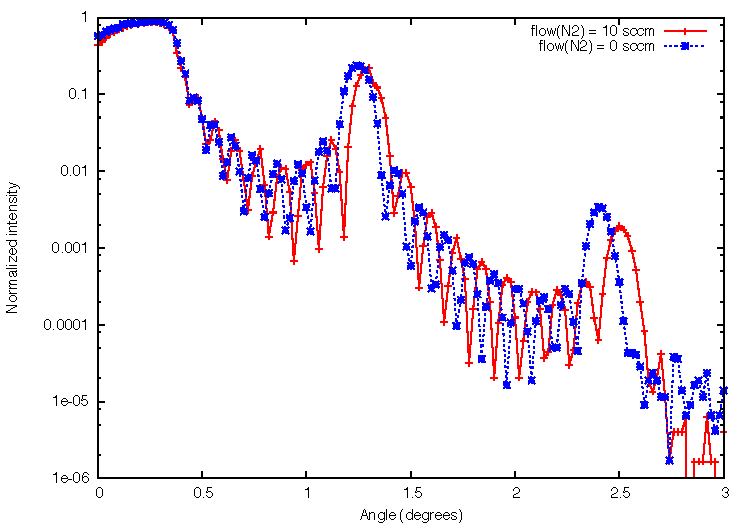
\includegraphics[width=0.47\linewidth]{figures/athena/coatings/w-b4c_n2_35AA.pdf}
	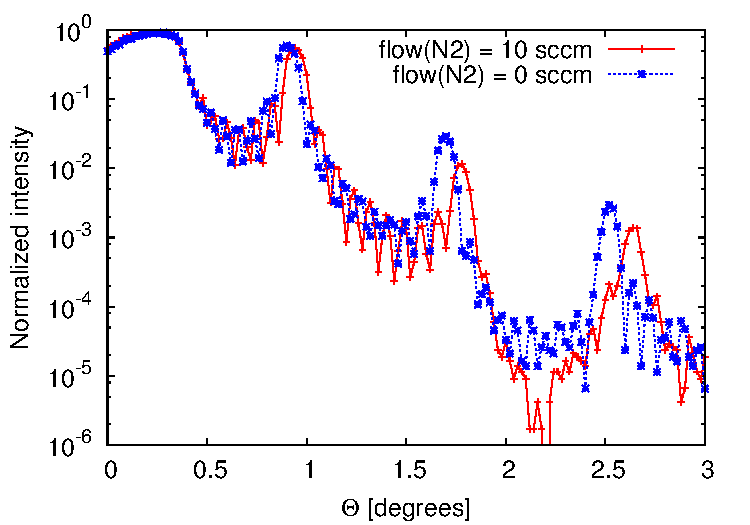
\includegraphics[width=0.47\linewidth]{figures/athena/coatings/w-b4c_n2_50AA.pdf}
\caption{\footnotesize XRR measurements of 10 bilayer W/B$_4$C coatings made with and without N$_2$ reactive sputtering (10 \% N$_2$, 90 \% Ar). \textbf{Left:} Coatings with a d-spacing of $\sim$3.5 nm. \textbf{Right:} Coatings with a d-spacing of $\sim$5 nm.}\label{fig:wb4c-n2}
\end{figure}

It was later found out from samples stored over time, that the coatings will visibly change over time if coated with N$_2$ reactive sputtering. A sample with discoloration can be seen in figure \ref{fig:discolor} (picture taken July 2014). The sample is a W/B$_4$C 10 bilayer calibration coating with a d-spacing of $\sim$5 nm. It was coated in February 2012 using 10 \% N$_2$ with 90 \% Ar at a total pressure of 2.9 mTorr.

\begin{figure}[!h]
	\center
	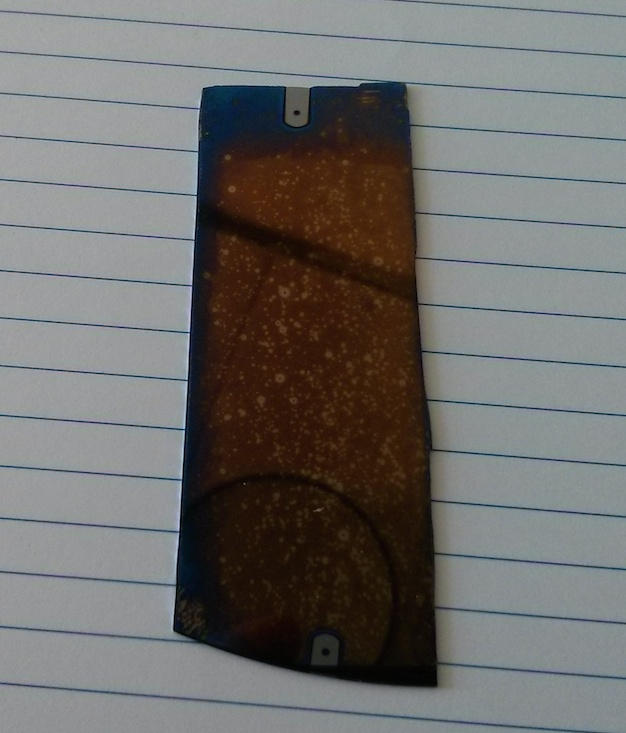
\includegraphics[height=5cm]{figures/athena/coatings/si5556.jpg}
\caption{\footnotesize Picture of sample coated with 10 bilayers of W/B$_4$C using N$_2$ reactive sputtering. Sample was coated in February 2012, picture taken July 2014.}\label{fig:discolor}
\end{figure}

Investigation into the literature gives a possible explanation. B$_4$C coatings react to humidity, but for BN coatings the effect is even more pronounced. The coating will absorb water molecules from the air, which diffuses through the coating and can eventually make the film peel off\cite{Cardinale:1994ha}. When B$_4$C coatings are sputtered with N$_2$ present, the nitrogen atoms become part of the film and will form B-N bonds. That would make all B$_4$C films produced with N$_2$ reactive sputtering deteriorate at ambient humidity. To test the hypothesis, a number of samples were produced with and without reactive sputtering, measured with XRR and subsequently placed in a desiccator at $\sim$20\% humidity.

The results can be seen in figure \ref{fig:wb4c-n2-storage}. The upper row are thick ($\sim$5.0 nm) and thin ($\sim$3.5 nm) samples of 10 bilayer W/B$_4$C coated with 10 SCCM N$_2$ flow ($\sim$10\% N$_2$). Middle row are samples with the same type and thickness of coating, but without N$_2$. Bottom row are also coated without N$_2$ but placed at ambient humidity ($\sim$45\%) outside the desiccator. The bottom row are also only stored for 3 months. The reactively sputtered coatings in the upper row show little change from Feb. 4th to June 28th, $\sim$5 months. What is interesting is the center row that show some interfacial changes in the film, especially for the thicker sample (left figure). Comparing to the bottom row, the thicker sample does not show the same changes over the 3 month period, but the thinner sample show significant change. The critical angle has shifted or washed out, the Bragg peak has widened and lowered in intensity. The sample also show visible discoloration, which is something that was not expected of a coating made without N$_2$ reactive sputtering. A more in-depth investigation into this problem is reported in section \ref{sec:long_term}.

\begin{figure}[htbp]
	\center
	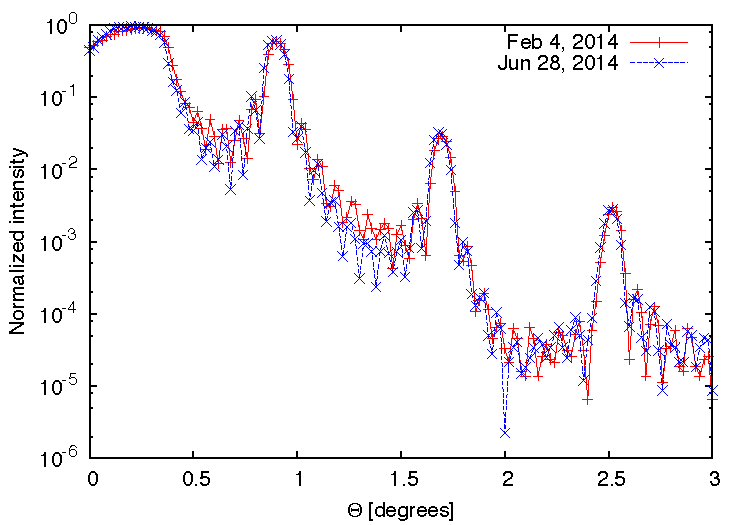
\includegraphics[width=0.47\linewidth]{figures/athena/coatings/w-b4c-n2-0sccm-thick.pdf}
	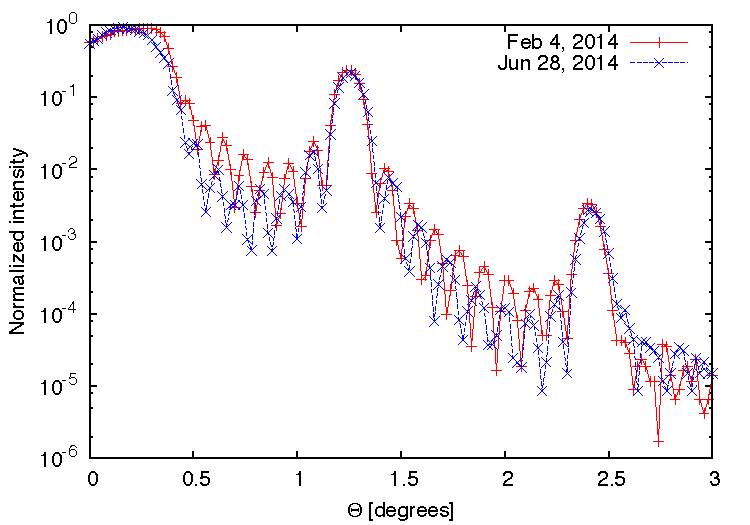
\includegraphics[width=0.47\linewidth]{figures/athena/coatings/w-b4c-n2-0sccm-thin.pdf}
	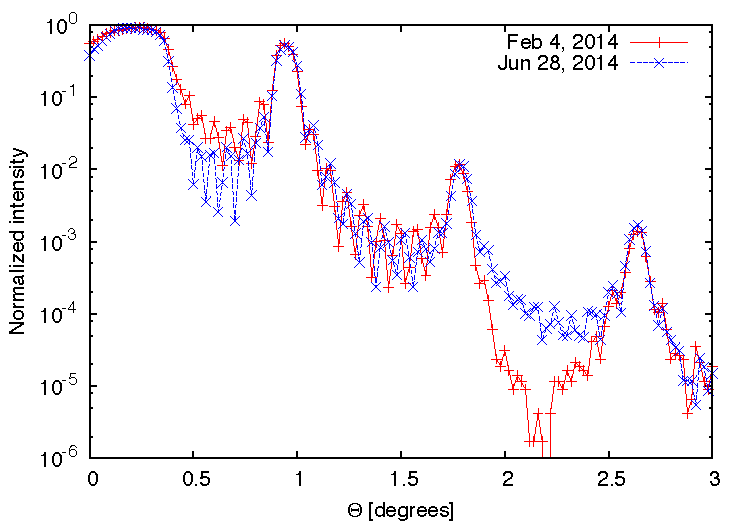
\includegraphics[width=0.47\linewidth]{figures/athena/coatings/w-b4c-n2-10sccm-thick.pdf}
	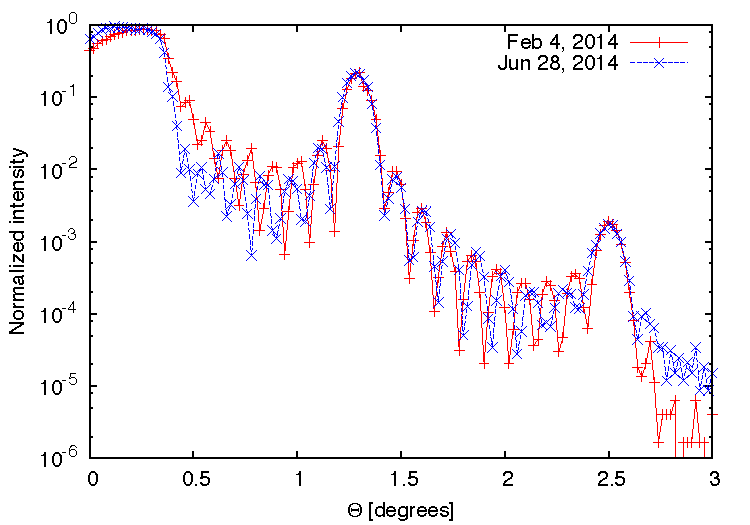
\includegraphics[width=0.47\linewidth]{figures/athena/coatings/w-b4c-n2-10sccm-thin.pdf}
	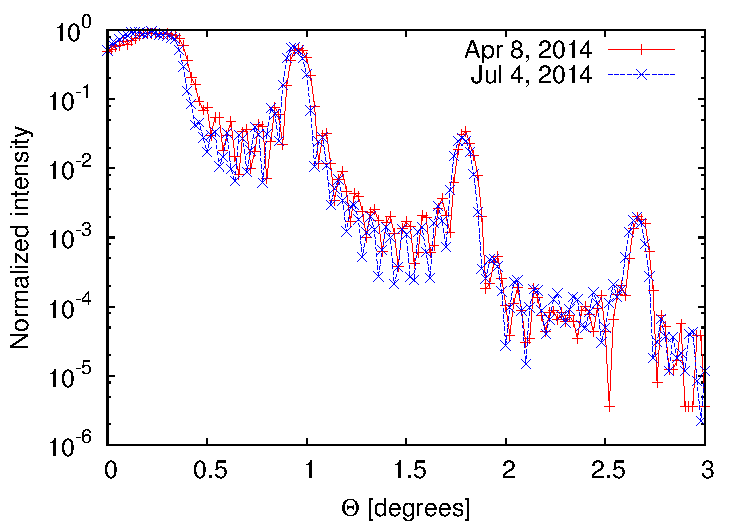
\includegraphics[width=0.47\linewidth]{figures/athena/coatings/w-b4c-no-storage-thick.pdf}
	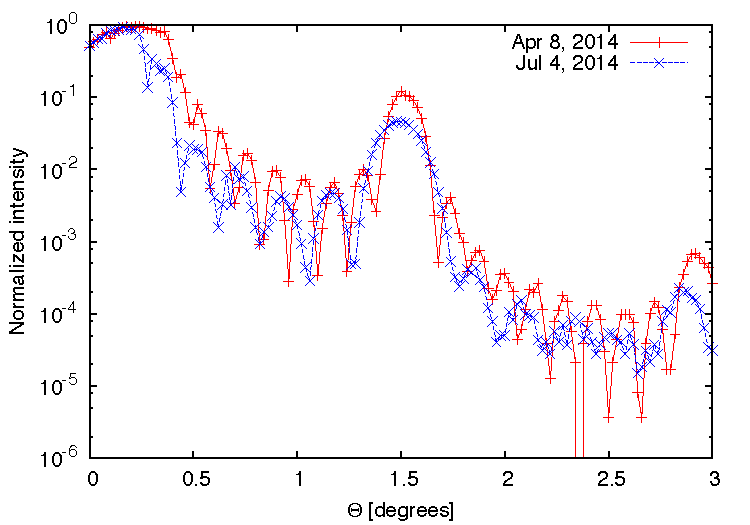
\includegraphics[width=0.47\linewidth]{figures/athena/coatings/w-b4c-no-storage-thin.pdf}
\caption{\footnotesize XRR measurements of samples coated with 10 bilayer W/B$_4$C films measured after coating and at a later time. Top and middle row samples were stored in a desiccator with $\sim$30 \% humidity. Bottom row samples were stored at ambient humidity ($\sim$50 \%).  \textbf{Top row} Samples coated with N$_2$ reactive sputtering (10 \% N$_2$, 90 \% Ar) and stored in desiccator, d-spacings of $\sim$5 nm (left) and $\sim$3.5 nm (right). \textbf{Center row} Samples coated with non-reactive sputtering and stored in desiccator, d-spacings of $\sim$5 nm (left) and $\sim$3.5 nm (right). \textbf{Bottom row} Samples coated with non-reactive sputtering and stored outside desiccator, d-spacings of $\sim$5 nm (left) and $\sim$3 nm (right) }\label{fig:wb4c-n2-storage}
\end{figure}

\begin{figure}[htbp]
  \center
  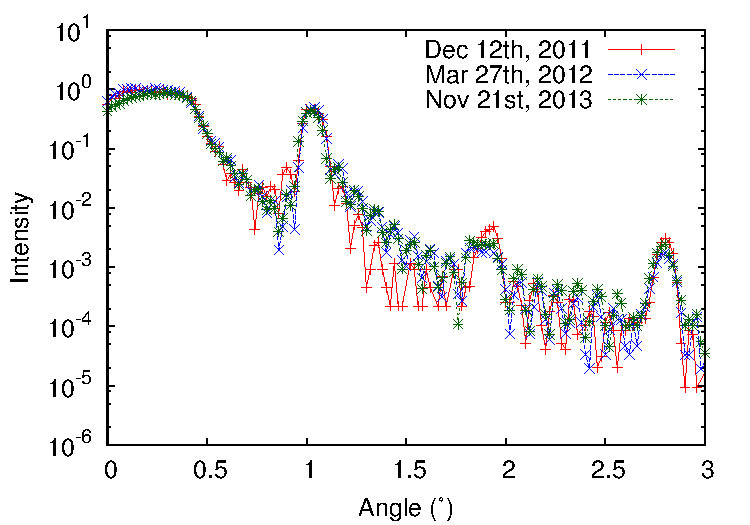
\includegraphics[width=0.47\linewidth]{figures/athena/coatings/pt-b4c-kalib2.pdf}
  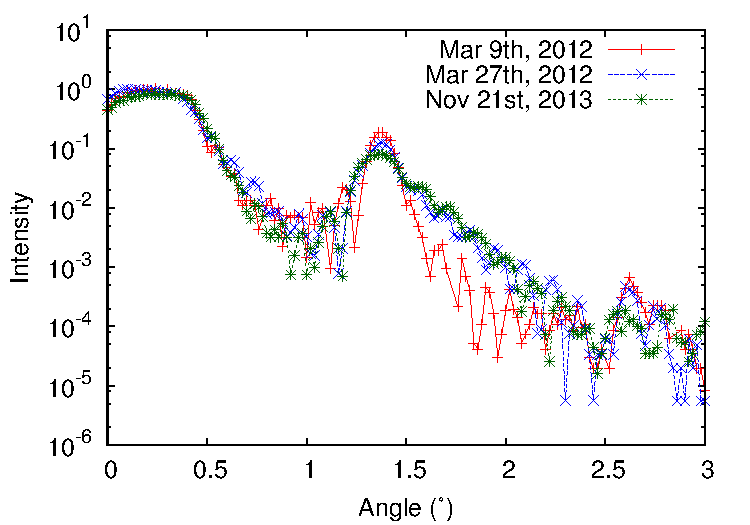
\includegraphics[width=0.47\linewidth]{figures/athena/coatings/pt-b4c-kalib1.pdf}
  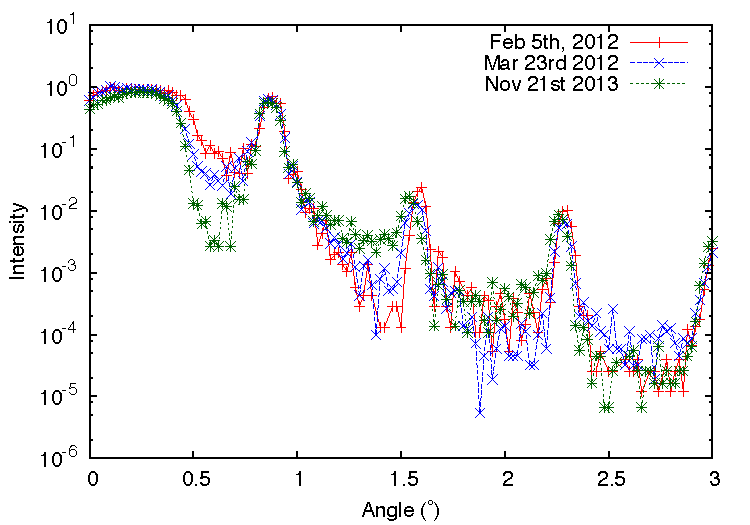
\includegraphics[width=0.47\linewidth]{figures/athena/coatings/w-b4c-kalib2.pdf}
  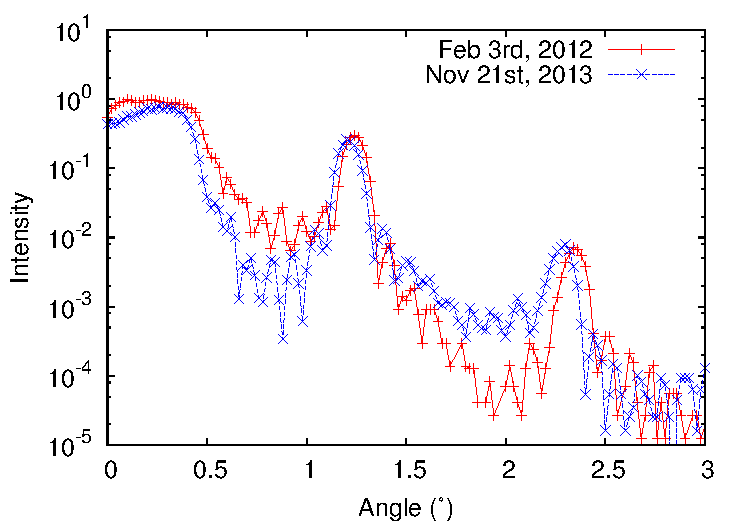
\includegraphics[width=0.47\linewidth]{figures/athena/coatings/w-b4c-kalib1.pdf}
  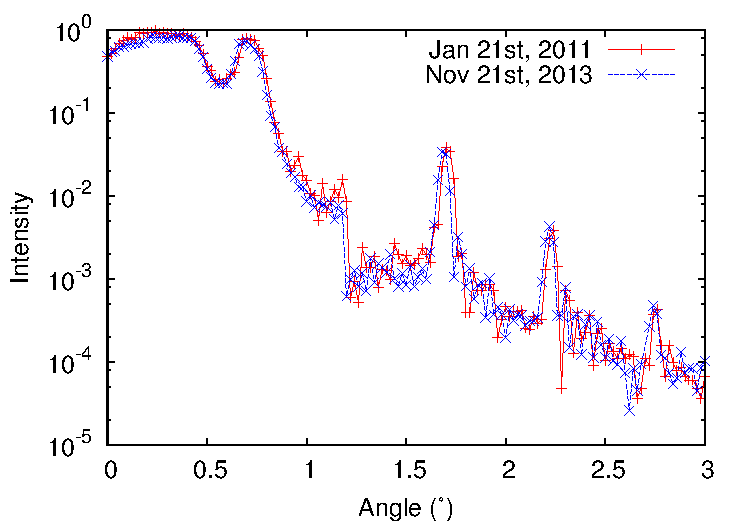
\includegraphics[width=0.47\linewidth]{figures/athena/coatings/ir-b4c.pdf}
  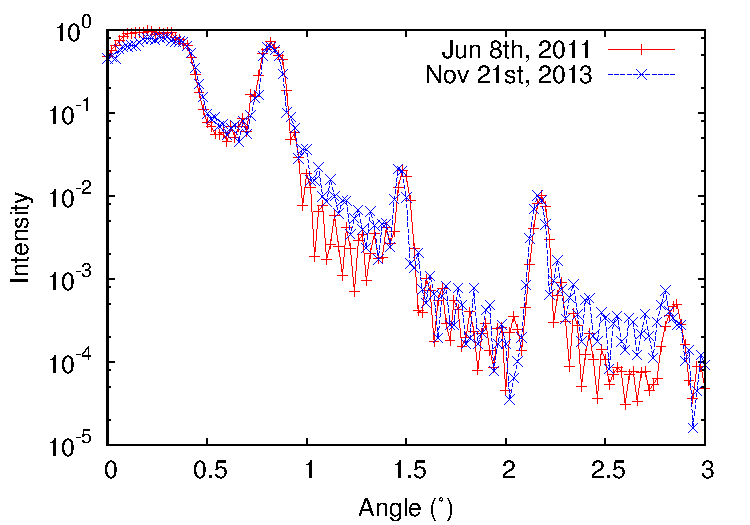
\includegraphics[width=0.47\linewidth]{figures/athena/coatings/ir-b4c-w-cr.pdf}
\caption{\footnotesize XRR measurements of coatings stored for 2-3 years at ambient conditions (outside desiccator).  \textbf{Top row} 10 bilayer Pt/B$_4$C with d-spacings of $\sim$5 nm (left) and $\sim$3 nm (right). \textbf{Center row} 10 bilayer W/B$_4$C with d-spacings of $\sim$6 nm (left) and $\sim$3.5 nm (right). \textbf{Bottom row} 10 bilayer Ir/B$_4$C with d-spacings of $\sim$8 nm (left) and 10 bilayer Ir/B$_4$C with d-spacings of $\sim$6.5 nm and a 10 nm Cr sublayer (right). }\label{fig:longtermstorage}
\end{figure}

\section{Long term storage investigation}\label{sec:long_term}
All samples coated at DTU Space are stored indefinitely for possible later investigation. The calibration samples of each material type for the ATHENA coatings are especially suitable for a long term investigation since the XRR measurement results of these samples have distinct features. In figure \ref{fig:longtermstorage} the results of XRR measurements of calibration samples are shown immediately after coating and after up to two years later. All the samples are coated without N$_2$ and using the standard Ar pressure of 2.9 mTorr.

In the upper row are shown 10 bilayer Pt/B$_4$C multilayers, middle row show W/B$_4$C multilayers and bottom row show Ir/B$_4$C multilayer (left) and Ir/B$_4$C multilayer with Cr sublayer (right).

The Pt/B$_4$C multilayers show significant change over time. The thicker film (left) show a rise in Kiessig fringe intensity between 1st and 2nd Bragg peak as well as a flattening of the 2nd Bragg peak. These effects show up already after $\sim$4 months. The thinner Pt/B$_4$C film (left) show even more deterioration, even after only 18 days. The 1st Bragg peak have widened and have grown a significant shoulder at higher angles.

The W/B$_4$C multilayers in the middle row also show significant change after less than two months. The thicker sample (left) have a shifted critical angle, corresponding to a change in $\Gamma$ in the multilayer. The thinner film (right) also show a change in critical angle, although less pronounced.

Ir/B$_4$C multilayers in the bottom row show very little change even after 2-2.5 years. The sample with Cr sublayer (right) shows some change in the Kiessig fringe intensity.

These results indicate serious problems in using B$_4$C films in certain material combinations. The baseline ATHENA coating of an Ir/B$_4$C bilayer and the alternative Ir/B$_4$C multilayer will according to these results be stable over longer periods of time.

\section{Coating of Ir/B$_4$C on SPO substrates}

\begin{figure}[!h]
  \center
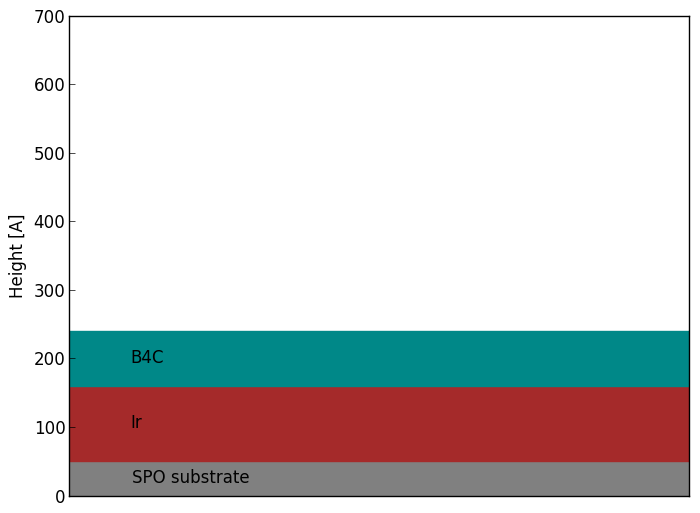
\includegraphics[width=0.4\linewidth]{figures/athena/coating_on_spo/ir-b4c-baseline.png}
  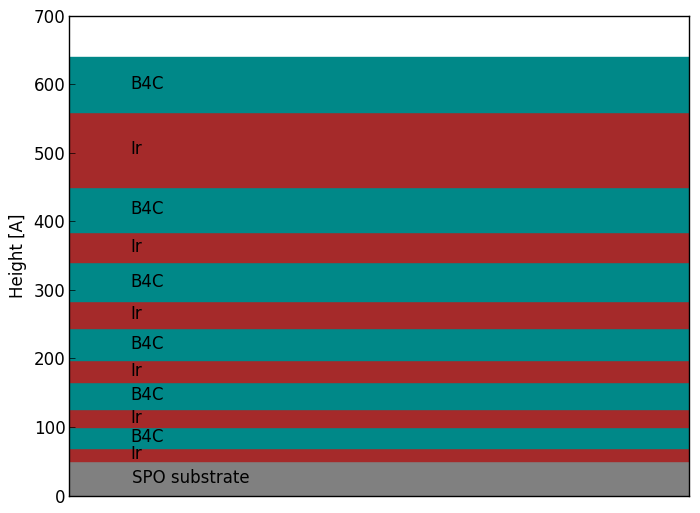
\includegraphics[width=0.4\linewidth]{figures/athena/coating_on_spo/ir-b4c-ml.png}
\caption{\footnotesize Side-view diagrams of Ir/B$_4$C coatings for ATHENA. \textbf{Left:} The baseline Ir/B$_4$C single bilayer. d$_{\text{Ir}} = 11.0$ nm,  d$_{\text{B}_4\text{C}} = 8.0$ nm. \textbf{Right:} The multilayer coating optimised for the middle part of the ATHENA optic. Consists of five bilayers with d$_{\text{min}} = 5.0$ nm, d$_{\text{max}} = 11.0$ nm, plus a cap layer of Ir of d$_{\text{Ir}} = 11.0$ nm and a top layer of B$_4$C of d$_{\text{B}_4\text{C}} = 8.0$ nm.}\label{fig:ml_baseline_sideview}
\end{figure}

\subsection{ISO qualification of Ir/B$_4$C coatings}\label{sec:qa_test}
In order to qualify the Ir/B$_4$C coatings on SPO substrates for the ATHENA mission, a range of tests were conducted on coated substrates. Four SPO substrates were coated, two with single bilayer baseline Ir/B$_4$C and two with optimised Ir/B$_4$C multilayer. The three tests were:

\begin{itemize}
 \item A thermal cycling test according to \emph{AD4 ECSS-E-10-03A (15 February 2002)}.
 \item A humidity test according to \emph{ISO9022(AD6)}.
 \item An adhesion test according to \emph{ISO9211-4(AD5)}.
\end{itemize}

A baseline and multilayer sample were used for both thermal cycling and humidity tests. The samples from the humidity tests were reused for the adhesion test. All tests were carried out by David Girou form DTU Space.

The thermal cycling test consists of eight cycles in a oven (no vacuum). One cycle is divided into two hours spent at $T_{max}=85$\degr C $\pm 10$\degr C and two hours spent at $T_{min}=-45$\degr C $\pm 10$\degr C. The test is divided into two times four cycles since reflectance measurements are performed after the fourth cycle. Figure \ref{4c} shows the temperature profiles for four cycles. Note that the temperature initial and final is 22\degr C, that $\dfrac{\text{d}T}{\text{d}t}=4$\degr C$\cdot$min$^{-1}$ and that after the last cycle the temperature is first increased to 40\degr C and then decreased to 22\degr C to avoid condensation. Reflectance measurements are done after the fourth and the eighth cycle.

\begin{figure}[!h]
  \center
  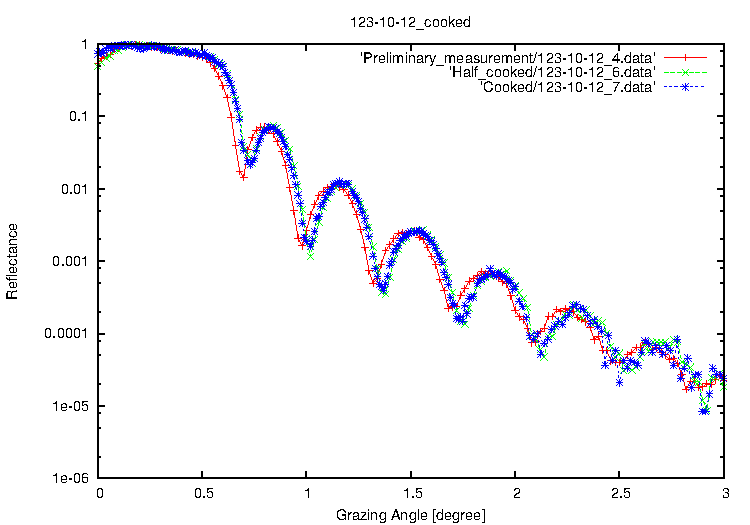
\includegraphics[width=0.47\linewidth]{figures/athena/coating_on_spo/123-10-12_cooked.pdf}
  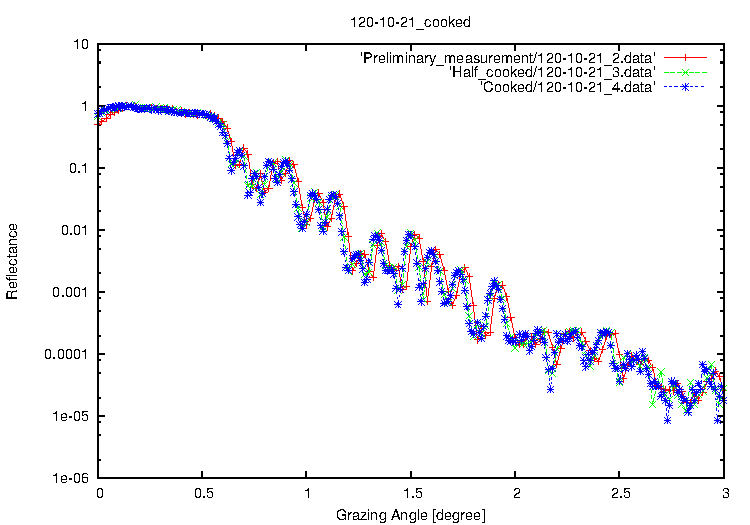
\includegraphics[width=0.47\linewidth]{figures/athena/coating_on_spo/120-10-21_cooked.pdf}
\caption{\footnotesize XRR measurements of Ir/B$_4$C coatings on SPO substrates before thermal cycling test, after four cycles, and after eight cycles. \textbf{Left:} Baseline Ir/B$_4$C coating. \textbf{Right:} Multilayer Ir/B$_4$C coating.}\label{fig:qa_temp}
\end{figure}

Results of the temperature test can be seen in figure \ref{fig:qa_temp}. No change is apparent apart from a misalignment of the first XRR measurement by 0.02\degr\ of both the baseline and multilayer (red lines).

The humidity test consists of 48 hours spent at a temperature of 40\degr C and a relative humidity between 90\% and 95\%. Samples are measured with XRR before and after the humidity test, results can be seen in figure \ref{fig:qa_hum}. No change in the baseline or multilayer XRR measurements after the humidity test.

\begin{figure}[!h]
  \center  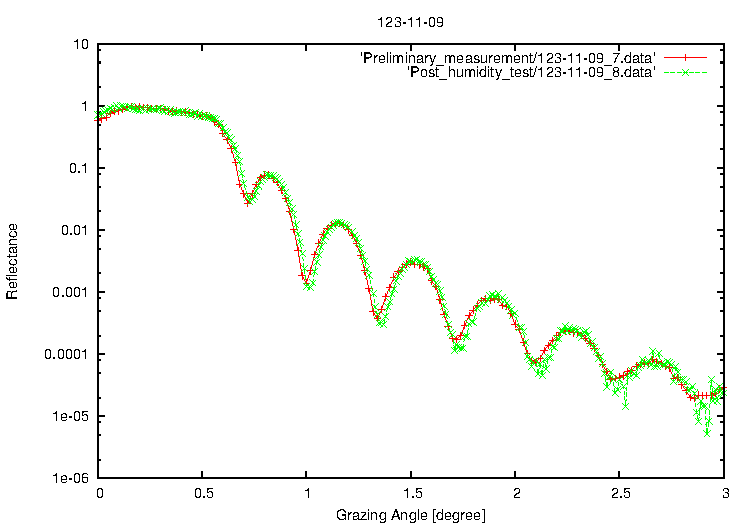
\includegraphics[width=0.47\linewidth]{figures/athena/coating_on_spo/123-11-09_Post_Humidity_test.pdf}
  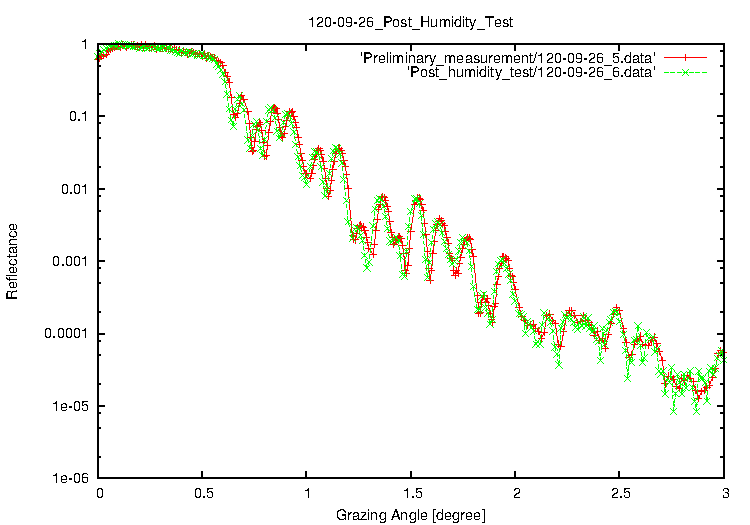
\includegraphics[width=0.47\linewidth]{figures/athena/coating_on_spo/120-09-26_Post_Humidity_Test.pdf}
\caption{\footnotesize XRR measurements of Ir/B$_4$C coatings on SPO substrates before and after a humidity test. \textbf{Left:} Baseline Ir/B$_4$C coating. \textbf{Right:} Multilayer Ir/B$_4$C coating.}\label{fig:qa_hum}
\end{figure}

The adhesion test was performed using a 25x19 mm$^2$ piece of scotch tape applied firmly to the surface of the coating on the SPO substrate. The tape was subsequently snapped rapidly off the surface. A visual inspection of the surface is performed afterwards. The degree of success of the test is measured in how rapidly the tape is pulled off without taking the reflective coating with it. No amount of pulling could remove neither the baseline nor multilayer Ir/B$_4$C coating. XRR measurements were also done on the samples to ensure that the top B$_4$C was not removed. As can be seen in figure \ref{fig:qa_adh}, both multilayer and baseline coating were unharmed in the test.

It is worth noting that the Ir/B$_4$C coatings applied to the SPO substrates were without a Cr underlayer to decrease the film stress. With that in mind, the Ir/B$_4$C baseline and multilayer can be expected to have had film stress of $\sim-$4 GPa and $\sim-$2 Gpa respectively[\ref{pap:PREL_ATHENA}].

\begin{figure}[!h]
  \center  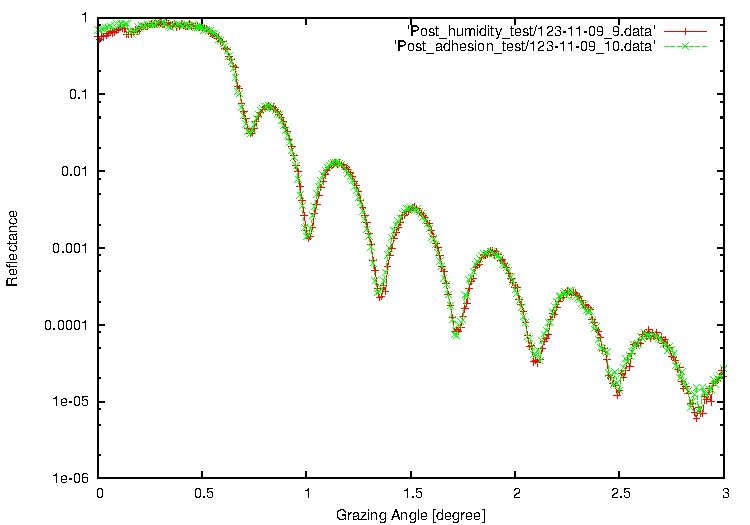
\includegraphics[width=0.47\linewidth]{figures/athena/coating_on_spo/123-11-09_Adhesion_test.pdf}
  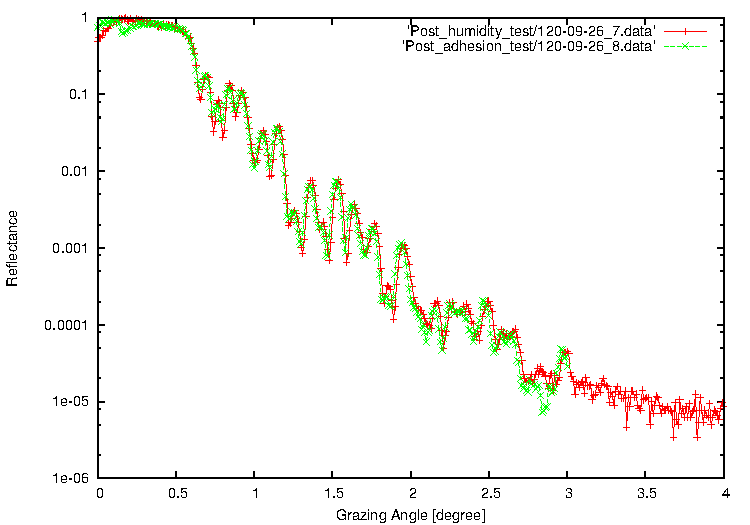
\includegraphics[width=0.47\linewidth]{figures/athena/coating_on_spo/120-09-26_Adhesion_test.pdf}
\caption{\footnotesize XRR measurements of Ir/B$_4$C coatings on SPO substrates before and after an adhesion test. \textbf{Left:} Baseline Ir/B$_4$C coating. \textbf{Right:} Multilayer Ir/B$_4$C coating.}\label{fig:qa_adh}
\end{figure}


\section{Upscaled production}\label{sec:athena_upscaled}

\emph{The following section was part of a technical report for the European Space Agency. It was done as part of the coating investigations for the original ATHENA proposed for ESA's L1 mission, which had a double-telescope configuration. It also required significantly less silicon pore optic substrates, 64,640 vs. $\sim$130,000 for ATHENA. The investigations done for scaling up production still holds true and the final production will also still take 2 years, but cost, production equipment and manpower will have to increase by a factor of two to three.}

For the ATHENA mission, the coating of the mirror substrates will be a large undertaking as 64,640 silicon pore optic (SPO) substrates will need a coating of between two and twenty layers.

Every piece will have to be transported from the SPO substrate fabrication facility (SFF) to a new dedicated coating facility, thoroughly cleaned, coated in specially designed chambers and then transported to the stacking facility. After stacking into mirror modules (MM), each MM will be measured at one of three dedicated beam lines at the BESSY II synchrotron in Berlin.

In this paper, an approximate cost and timeline of the coating and coating qualification of SPO substrates is given.

\subsection{Timeline and cost of procurement and setup of coating facility}

Cleaning and coating of SPO substrates will require as a minimum an ISO 7 clean room to avoid dust particles. Dust on the substrates before coating will result in small holes in the coating, which will reduce the effective area. There are two possibilities for the location of the coating facility which is discussed in this paper. Either the facility is located in the same building or adjacent building as the stacking facility or the coating facility is placed further away, i.e. another country within Europe.

Moving substrates in and out of clean rooms and transporting them over larger distances has drawbacks and extra costs associated. But locating the two facilities separately can reduce costs as it will be easier cheaper to find two smaller clean rooms to re-purpose into production facilities. Building and setting up clean rooms of a sufficient size for both facilities will take several years and come with a significant cost, but if it is possible to re-purpose existing laboratories that cost can be reduced.

The first part of the clean room should be for opening shipments from the SFF and cleaning each substrate. As the substrates are produced in a clean room at the SFF, it is assumed that they will at maximum need to be cleaned with an air gun with dry nitrogen. After being cleaned, each substrate is mounted onto a substrate holder that will be inserted into a coating chamber for coating. When the coating is done, the substrate holder is taken out of the chamber and the substrates are ready to go into the stacking facility.

Clean rooms can be build inside existing larger storage areas or cleaner production facilities. The approximate timeline for the setup of the entire facility is as follows:

\begin{description}[itemsep=1.5pt,parsep=1pt]
	\item[9] \textbf{years before launch:}
		\begin{itemize}[itemsep=1.5pt,parsep=1pt]
		\item[-] Planning begins for the construction of a shared cleanroom facility.
		\item[-] Planning begins for coating chambers.
		\end{itemize}
	\item[7-8] \textbf{years before launch:}
		\begin{itemize}[itemsep=1.5pt,parsep=1pt]
		\item[-] Construction of facility is carried out.
		\item[-] Produced coating chambers are installed and qualifications begun.
		\end{itemize}
	\item[6] \textbf{years before launch (CDR):}
		\begin{itemize}[itemsep=1.5pt,parsep=1pt]
		\item[-] Coating capabilities ready.
		\end{itemize}
\end{description}

The cost of building and preparing the coating facility will differ between a shared facility and separated facilities, but the coating chambers will have a similar configuration.

\subsection{Coating chambers}\label{sec:chambers}
The two telescopes of ATHENA consists of 64,640 SPO substrates, which are all coated. Considering the coating chamber design used at DTU Space, a maximum of 100 plates can be coated per day in an 8 hour workday. In a year of 200 workdays, 20,000 substrates can be coated. Using three chambers, 60,000 substrates can be coated per year, within the two year time frame a total of 120,000 substrates can be coated. A minimum of 90,000 coated is considered as baseline, as we account for damaged plates, bad coatings etc. That leaves an acceptable down time of 6 months throughout the project.

Using chambers of same design as DTU Space will give a cost of around 1M \euro\ per chamber. Those chambers have the drawback of a long pump down time after having the chamber opened to change samples. The advantage of coating SPO substrates compared to e.g. NuSTAR glass is that the SPO substrates are flat and only $\sim$1 mm thin.

If a new chamber design is considered, it would be advantageous to pursue a design similar to what is used in the semiconductor industry. Here an entire wafer are given a number of different coatings and automatically moved from one cathode to another using a robotic arm. As those wafers can have a thickness of up to 3 mm, we propose to use a substrate holder shaped like a wafer 3 mm thick with a diameter of 300 mm. Recessions in the substrate holder can accommodate SPO substrate and no clips will be needed to hold substrates in place, since the wafer will at all times be horizontal. A chamber of that design will not need pump down time between each batch of substrates, since wafers will be inserted into the central vacuum chamber through a narrow slit directly from a clean magazine in atmospheric pressure. Every coating cathode is also in a separate chamber and can be accessed without venting the entire machine. Custom made machines like seen in figure \ref{fig:dram} are priced at $\sim$2M \euro.

\begin{figure}[htbp]
	\centering
		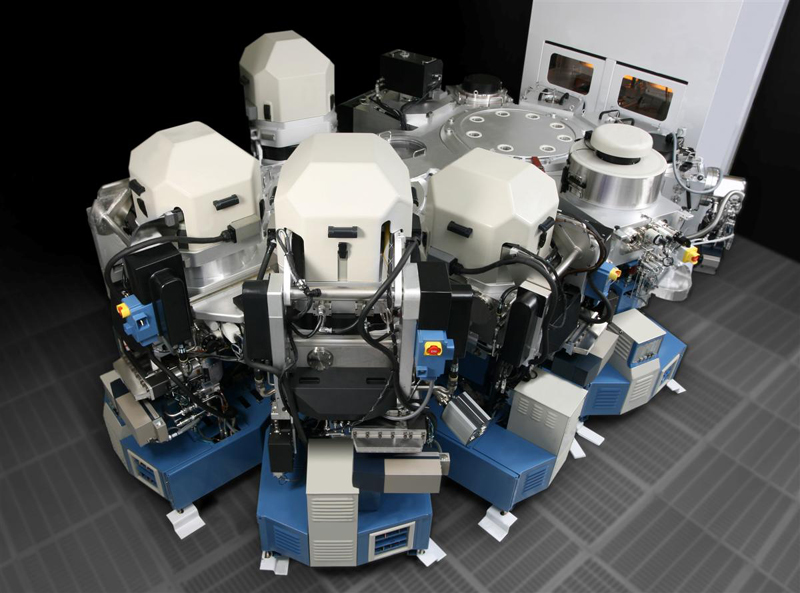
\includegraphics[width=0.6\textwidth]{figures/athena/dram.jpeg}
	\caption{\footnotesize Multi-chamber deposition machine from Applied Materials. \emph{Source: www.appliedmaterials.com}}
	\label{fig:dram}
\end{figure}

A significant increase in production rates can be achieved using machines like this. It also gives a cleaner environment for samples, since the machine itself can stay closed for longer periods of time. Higher production rates means that only one or two chambers are needed to complete the coating of 90,000 SPO substrates in two years.

\subsection{Shared facility}
Since both the coating facility stacking facility needs a clean room, these can be combined or connected in a shared facility. If the chamber design from DTU Space is used, a separate clean room will be needed to accommodate these chambers as they can give off dust flakes of material every time they are opened. If instead a multi-chamber coating system is used as described in section \ref{sec:chambers}, the coating machinery can be in a separate clean room against the wall into the stacking facility. That way wafer cassettes full of wafer-shaped SPO substrate holders can be inserted and retrieved from the stacking facility clean room.

For a shared facility with multi-chamber coating systems as described in section \ref{sec:chambers}, we propose the following facility setup:

\begin{itemize}
	\item Common class 10,000 clean room for mounting SPO substrates on wafer-shaped sample holders. The same room will be used for fast X-ray system for pre- post coating measurements.
	\item Access to insertion port of multi-chamber coating system from the common clean room. Wafer cassettes are mounted directly to accessible part of the machine.
	\item The back end of the coating chambers are in a separate room, so targets can be changed without giving off dust near the substrates.
	\item In connection to the common clean room is a separate class 100 - 10,000 clean room with stacking robots. The robots can be in a separate ventilated tent inside the clean room to decrease particle dust. Mirror modules will be sealed here and moved outside the clean rooms for packing and shipping to BESSY II.
\end{itemize}

\subsection{Separated facilites}
If the facilities are separated, a large effort will be required to keep substrates clean when packing/unpacking for transport. The substrates will be send from the SFF in batches of 1,500 and double or triple sealed, so the package can be opened partly when inside a moderately clean room opened completely in the main class 10,000 clean room. The following setup of clean rooms is proposed.

\begin{itemize}
	\item Two separate class 10,000 clean rooms, one for substrate handling and one for coating chambers. Alternatively, one larger clean room parted by a clear plastic curtain.
	\item Substrate handling clean room will also be used for the fast X-ray system for pre- and post coating measurements.
	\item Coated samples will be packed and double sealed inside the clean room before being shipped to the stacking facility.
\end{itemize}

\subsection{Resist deposition and removal at alternative facility}
One of the processes done at the SFF to the substrates before sending them to the coating facility will be the lithographic process of resist deposition. It requires a semiconductor grade facility to apply the resist using spray-on and afterwards removing stripes by a UV radiation process.

The process can, instead of at the SFF, be done either at the coating facility by including the proper equipment or at an external facility. DTU Danchip is the Danish National Center for Micro- Nanofabrication, which runs a class 10 clean room with equipment capable of depositing the resist and UV curing the SPO substrates.

The removal of the resist after coating can be done at the stacking facility, but can instead be done at the coating facility if these are separated. By doing the resist removal at the coating facility, a visual inspection can be done of the substrate before being transported to the stacking facility. If the process damages the coating, the problem can be located and new coated substrates can be produced quickly.


\subsection{Cost for setting up}
To prepare the lab before the coating campaign starts, the coating chambers will need to be installed and configured. An extensive campaign with scientific personnel is needed to ensure the system's capability to produce coatings of sufficient quality. We estimate 12-24 months to qualify the coating chambers for the ATHENA coating campaign and will need approximately two scientific personnel and one technician.

The coating qualification equipment described in section \ref{qualification} will be needed to qualify the coating chambers.


\begin{table}[htbp]
	\centering
\begin{tabular}{l|c}
Equipment & Approx. price \\
\hline
\hline
3 x Coating chambers of DTU design  & 3 x 1,000,000 \euro\\
\hline
or:\\
\hline
2 x Multi-chamber coating systems & 2 x 2,000,000 \euro \\
\hline
\\
\hline
Personnel for setup & 490,000 \euro\\
\end{tabular}
\end{table}


\subsection{Timeline and cost for production of ATHENA coatings}
SPO substrates are fabricated at the SFF and should be shipped to the coating facility weekly in shipments of 1500 substrates. 300 substrates are daily mounted on wafer shaped sample holders after they have been measured using the fast X-ray system. The substrates are coated in one of the coating chambers and subsequently taken out to have resist removed and be measured again using the fast X-ray system.

Cost drivers during production are sputtering targets and personnel. The final cost is dependent on which material combination is used for coating. The differences can be seen below.

\begin{table}[htbp]
	\centering
\begin{tabular}{l|c|c|c|c}
Material 	& High Z 		& Approximate & Low Z  & Approximate \\
combination & thickness & price / mm$^3$ & thickness &  price / mm$^3$ \\
 & (nm) & (High Z) & (nm) &  (Low Z) \\
\hline
\hline
Cr/Ir/B$_4$C & 10 & 10.9 \euro & 8 & 0.26 \euro\\
\hline
Pt/B$_4$C & $\sim$16 & 10.5 \euro & $\sim$22 & 0.26 \euro\\
\hline
W/B$_4$C & $\sim$16 & 0.73 \euro & $\sim$22 & 0.26 \euro\\
\end{tabular}
\end{table}

The approximate cost is calculated based on a 10\% efficiency of the sputtering cathodes, meaning 10\% of the target material ends on a substrate. For a single layer of 10 nm on all the substrates of ATHENA, the volume of material needed will be approximately 5 cm$^3 = $ 5000 mm$^3$. From that, the total target cost can be estimated.

\begin{table}[htbp]
	\centering
\begin{tabular}{l|l|c|c}
Material 	& Type of coating & Approx. cost & Approx cost incl. \\
combination	&	&	&	30 \% target \\
&	&	&	usability\\
\hline
\hline
Cr/Ir/B$_4$C & Tri-layer & 57,000 \euro & 190,000 \euro \\
\hline
Pt/B$_4$C & Graded-d multilayer & 87,000 \euro & 290,000 \euro\\
\hline
W/B$_4$C & Graded-d multilayer & 8,700 \euro & 29,000 \euro \\
\end{tabular}
\end{table}

Only 30\% of the target can be used before it has to be replaced, so a factor of 3-4 should be applied to these cost estimates. The leftover targets of precious metals, platinum and iridium, can be sold back at market value, which can reduce the total costs of precious metal consumption by up to $\sim$50 \%.

For a Pt/B$_4$C graded-d multilayer, the total thickness of Pt is 16 nm in average and 22 nm of B$_4$C. Thus, $1.6 \cdot 5000$ mm$^3$ of Pt is needed at a price of 10.5 \euro\ per mm$^3$ at 90 \% coating loss, combined with $2.2 \cdot 5000$ mm$^3$ of B$_4$C at 0.26 \euro\ per mm$^3$ gives a total cost of 87,000 \euro.

\subsection{Personnel}
During the two year coating campaign, 300 substrates will be handled daily. Procedures to be done daily include:

\begin{itemize}[itemsep=1.5pt,parsep=1pt]
	\item Unpacking substrates.
	\item Measuring using fast X-ray system.
	\item Mounting substrates on sample holders.
	\item Load sample holders in coating chamber.
	\item Running coating equipment.
	\item Unloading sample holders.
	\item Remeasuring using fast X-ray system
	\item Repacking samples for transport to stacking facility.
\end{itemize}

Additionally, the coating chambers will require new targets to be installed on a weekly basis. We estimate 3-4 technicians are needed in addition to 2-3 scientific personnel to run the coating production.

For three technicians two scientists, a two year coating campaign will cost 1,400,000 \euro.

%\subsection{Shared facility}
%\subsection{Separated facilites}

\subsection{Coating QA during production}\label{qualification}
We envision a significant coating qualification campaign for the ATHENA mission. We propose a fast automated 8 keV X-ray setup, that can measure every plate before and after coating. The plan is to make reflectivity scan of ca 50 \% of the pores.  Each measurement is an angular scan  at a fixed 8 keV energy and at an angular range of 0\degr to $\sim$ 1.5\degr\ will determine micro roughness to an accuracy of +/- 0.02 nm. It till require automatic alignment to an accuracy of +/- 0.01\degr. Measurements for each plate should be conducted in less than 5 minutes and each scan should be automatically fitted, with the data logging and plotting part of the facility. The foot print of the beam should cover more than 10 \% of each pore.

The total database of reflectivity measurements can be used when building the final optical response model for ATHENA. During the campaign it will be required to measure ~600 SPO substrates per day, so the system should be capable of measuring each substrate in a batch automatically.

Every chamber needs to be calibrated twice a week to ensure a precise layer thickness. This will require samples to be coated with constant-d multilayers, which will be measured using a separate 8 keV X-ray reflectivity (XRR) setup at the facility.

In every coating run, a witness sample will be included along with SPO substrates. These witness samples will be measured using the 8 keV XRR setup to ensure proper layer thickness interfacial roughness. In addition, 5x70 mm wafer pieces are also coated measured for stress using a stylus measurement tool. One or two times a week, a coated SPO substrate will be taken out to check for adhesion and visual QA in a microscope. If contamination is suspected, an AFM analysis will be carried out, if necessary externally.

Measuring samples at the energies visible by ATHENA can help build the final optics model. We propose this optional addition: A single coated substrate per day will be selected for reflectivity scatter measurements at the BESSY II synchrotron at PTB Berlin. 25 substrates per month can be measured using X-ray reflectivity energy scans at 4 to 10 keV at BESSY II within 2-3 days. A few more days per month will be needed to measure scattering from select substrates.

Below are approximate prices for equipment needed.

\begin{table}[htbp]
	\centering
\begin{tabular}{l|c}
Equipment & Approx. price\\
\hline
\hline
Fast automated 8 keV X-ray setup  & 1,000,000 \euro\\
\hline
Separate 8 keV X-ray setup & 500,000 \euro\\
\hline
Stylus stress measurement setup & 30,000 \euro\\
\end{tabular}
\end{table}



\subsection{Timetable and cost}

The timetable is independent on whether the coating facility is shared with the stacking facility or separate.\\

\begin{table}[htbp]
	\centering
\begin{tabular}{c|l}
T - 9 years & Planning begins for the construction\\
  & \hspace{1cm} of a shared clean room. \\
			& Planning begins for coating chambers.\\
\hline
T - 8 years & Construction of facility is carried out.\\
			& Produced coating chambers are installed\\
      & \hspace{1cm} and qualifications begin.\\
\hline
T - 7 years & Continuation of coating chamber qualifications.\\
\hline
T - 6 years & Coating chamber qualifications complete.\\
			& Coating capabilities ready.\\

\end{tabular}
\end{table}

The timetable gives the possibility of starting the coating campaign six years before launch. The coating campaign is set for two years including delays will have the optic ready four years before launch. The four year window between optic readiness and launch is specified in the ESA timetable.

Total cost for a shared facility is calculated below. For a separate facility, transport costs of substrates will have to be included, estimated at 100,000 \euro. Substituting three DTU design coating chambers with two more advanced multi-chamber systems will increase the cost of coating chambers to 4 mio. \euro.

\begin{table}[htbp]
	\centering
\begin{tabular}{l|c}
Expense & Approx. price\\
\hline
\hline
3 x Coating chambers of DTU design  & 3 x 1,000,000 \euro\\
\hline
or:\\
\hline
2 x Multi-chamber coating systems & 2 x 2,000,000 \euro \\
\hline
\\
\hline
Fast automated 8 keV X-ray setup  & 1,000,000 \euro\\
\hline
Separate 8 keV X-ray setup & 500,000 \euro\\
\hline
Stylus stress measurement setup & 30,000 \euro\\
\hline
Sputtering targets & 300,000 \euro\\
\hline
Personnel during setup & 1,000,000 \euro\\
\hline
Personnel during production & 1,400,000 \euro\\
\hline
\textbf{Total} & $\leq$ 8,230,000 \euro\\
\end{tabular}
\end{table}

\section{ATHENA discussion and conclusion}
The ATHENA mission is set to launch in 2028 and it is clear that many things has to fall into place to meet the deadline, especially the large production effort that has to be realised. From the results in described in this chapter, the choice of Ir/B$_4$C material combination seems to be the only possibility to meet the target of 2 m$^2$ effective area at 1 keV. An alternative material combination that could work with the lithographic process described in section \ref{sec:athena_opt_tech} is W/Si, but the higher electron density of Si would seriously impact the effectivity at lower energies and so would the absorption edge of Si at $\sim$1.8 keV.

Selecting B$_4$C as the low-Z material in the reflective coating is an obvious choice considering for an X-ray telescope with sensitivity down to 0.1 keV, but as this chapter shows, there are serious problems with B$_4$C in combination with Pt or W. Reflective W/B$_4$C multilayer coatings for X-ray purposes has been reported in the litterature\cite{Jankowski:1991kx,Morawe:2007vp}, but none has shown the long term effect ambient conditions can have on these coating. Some report on the stability of W/B$_4$C multilayers after heat treatment to 500\degr C\cite{JANKOWSKI:1990vd} or 800\degr C\cite{Rao:2013dt}, but both were done under vacuum ($<10^{-4}$ Torr).

Extensive investigations in the literature has shown no reports on the deposition of a Pt/B$_4$C multilayer combination, so this chapter provides the first measurements of the coating and long term stability. The multilayers were found to have a high interlayer roughness by XRR immediately after coating, so it was decided to use a single Pt/B$_4$C bilayer as a backup solution to the Ir/B$_4$C baseline because of the lower stress. However, the long term stability tests revealed what seems to be a large amount of diffusion at the Pt/B$_4$C interface, leading to a break-down of the multilayer structure. Even in a single bilayer film the high amount of diffusion will significantly increase interlayer roughness over time.

The changes in both Pt/B$_4$C and W/B$_4$C over time seems to be only under ambient humidity, i.e. not an issue after launch; but keeping every single coated SPO substrate out of humidity for 4--6 years during production and until launch is not quite realistic. The end result is a complete disqualification of both Pt/B$_4$C and W/B$_4$C for ATHENA in favor of Ir/B$_4$C single bilayer or multilayers and with W/Si as a backup solution, although without meeting science requirements of 2 m$^2$ at 1 keV effective area.

The qualification tests of Ir/B$_4$C coatings on SPO substrates described in section \ref{sec:qa_test} showed great promise in the stability of the material combination even under high humidity and temperature. Later tests were done to see how high a temperature the coatings can withstand before breaking down, but even several hours at 300\degr C showed no change in structure in XRR measurements. The high stress of the materials that was seen early in the investigations can be mitigated using a Cr underlayer, and the high surface roughness of Cr can be mitigated by a unique smoothening effect of Ir. Even without a Cr underlayer, it seems that the high stress has no consequence on the stability of the coatings; and as the SPO substrates are extremely stiff, no bending is likely to occur as a result of film stress.

The choice between single bilayer or multilayer Ir/B$_4$C coatings for ATHENA is a question of cost. Applying a single bilayer is the inexpensive solution, as it puts the least requirements on production facilities; every SPO substrate will get the same coating. Multilayers of 5--10 bilayers will require more time per sample to apply as well as more complicated coating chambers. One could imagine a linear coating system with one Ir cathode and one or two B$_4$C cathodes, SPO samples would enter in one end of the system and exit in the other end, thereby finishing a baseline single bilayer coating with just a linear movement through the chamber. A similar setup for multilayer coatings would require a system with up to 20 cathodes in a row of interchanging Ir and B$_4$C, a massive system with multiple points of failure. An alternative approach is the multi-chamber solution as described in section \ref{sec:chambers}, which is the recommended solution reported to ESA by DTU Space. The multi-chamber coating facility takes advantage of the SPO technology heritage from the semi-conductor industry, primary advantage being the completely flat geometry of SPO substrates before stacking.

The past decades of rapid growth and technological progress in the semi-conductor industry will definitely be a major reason for making a telescope with more than 120,000 mirror substrates possible. A similar sized mission with individually slumped glass substrates as in the NuSTAR mission will require a substantial man-power effort as each step from flat glass to curved, cleaned and coated glass mirrors are labor-intensive and almost impossible to automate. The SPO technology has drawbacks, such as limits on material combinations and a larger minimum inner radius compared to slumped glass, but the low substrate figure error, mass production capability, and rigidity of mirror modules gives SPO a substantial advantage in large X-ray missions.
